%! TEX root = ../outline.tex

In this chapter the univariate distribution reconstruction from quantiles, copula parameter fitting, Monte Carlo and importance sampling strategies are exercised with a synthetic data set.  Synthetic data offers advantages over CFD born data for the purposes of testing and evaluating the efficacy of the proposed models.  

The synthetic data conforms to a known functional form with specified distribution and bias parameters. These properties are useful for benchmarking and validation investigations which seek to ensure that the fitted models retain key statistical properties from the synthetic data set. This chapter does not introduce machine learning components and does not explore forward model predictions.  %See chapter \ref{sec:ml_cfd} for hi2lo model performance when used in a predictive capacity.

The availability of synthetic data alleviates the need to generate comparatively expensive CFD results to test the hi2lo strategy.  Some aspects of CFD fields are preserved in the synthetic data, including expected biases between CFD and CTF results that arise due to discrepancies in wall heat transfer closure models, among other differences.  Turbulent dispersion of the temperature and near wall TKE distributions around spacer grids are emulated by the synthetic data model.  Additionally, the dependence structure between the cladding surface temperature, boundary heat flux, and near wall TKE may be enforced by the synthetic data generation tool.  Accounting for spatial auto-correlation in the surface fields was not pursued.    Consequently the synthetic data is not a direct replacement to CFD data but serves as data source for method interrogation and integration testing.

The joint distribution model comprised of a copula and quantile functions are fit to the synthetic data in each CTF face independently.  The number of quantiles used to reconstruct the quantile functions is a user controllable quantity, and was set to 20 in this case.  Samples are drawn from the fitted joint temperature, TKE and BHF density models on each patch using standard Monte Carlo methods or importance sampling.  The surface samples are provided to a crud simulation package as cladding-surface boundary conditions.  Additional required bulk coolant properties such as the bulk fluid temperature and bulk concentration of soluble boron are supplied by CTF.

Time dependent crud simulation is also discussed.  The interaction between the sample surface remapping strategy and the integrated crud results are discussed.  Furthermore, the process by which importance sample weights are averaged over discrete time steps is discussed.

Speedups afforded by importance sampling are presented and contrasted against standard Monte Carlo sampling results.  The sampling distributions utilized in importance sampling are informed by the physics of crud growth.

\section{Generating Synthetic Data}
\index{Synthetic CFD Data}

Synthetic data generation begins by running standalone CTF on a single quarter symmetric pin.   The CTF result is then augmented with tailored noise.  The augmented synthetic surface fields may be constructed by equation \ref{eq:synth_aug}.
\begin{align}
    \bm X &= \bm \mu_{ctf} + \bm b + \bm \varepsilon \nonumber \\
          &=
    \begin{pmatrix}
        T \\
        k \\
        q''
    \end{pmatrix}
    =
    \begin{pmatrix}
        \mu_{T} \\
        \mu_k \\
        \mu_{q''}
    \end{pmatrix}_{ctf}
    + \begin{pmatrix}
        b_{T} \\
        b_k \\
        b_{q''}
    \end{pmatrix}
    + \bm{\varepsilon} (\mathbf z; \bm \theta),
\label{eq:synth_aug}
\end{align}
Where $\bm \varepsilon(\mathbf z, \bm \theta)$ is a user controlled spatially dependent residual random vector with a mean of 0.  This residual is
shifted by a bias vector
$\mathbf b$ and where $\mathbf z$ is the axial and azimuthal location on the rod surface.
$\bm \theta$ represents user specified distribution parameters.

Equation \ref{eq:synth_aug} represents three continuous random surface fields.  In practice a large number of independent and identically distributed samples are drawn in each CTF face from the underlying random field.  Individual surface samples may be specified by equation \ref{eq:synth_aug_discrete}.

\begin{equation}
    X_{ij} = \mu_{j,\mathrm{ctf}} + b_j + \varepsilon_{ij};\ \   \varepsilon_{j} \sim h_j
    \label{eq:synth_aug_discrete}
\end{equation}
Where the index $j$ represents the $j^{th}$ CTF face on the rod, and the index $i$ is the sample index within the $j^{th}$ CTF face.  The distribution parameters are constant over a given CTF face and are represented by $\bm \theta = \{\theta_c, \{\theta_x\}\}$ where $\theta_c$ is the copula parameter and  $\{\theta_x\}$ are the set of marginal distribution parameters.

Shown in equation \ref{eq:synth_aug_face}, according to Sklar's theorem the surface residual temperature and TKE joint distribution may be decomposed into copula an marginal models on each CTF face:

\begin{equation}
    h_j = c_j(F_k(k), F_T(T); \theta_{c_j}) f_{T}(T; \theta_{T_j}) f_{k}(k; \theta_{k_j})
    \label{eq:synth_aug_face}
\end{equation}
Where the copula parameter $\theta_{c_j}$ and the marginal temperature and TKE distribution parameters $\theta_{T_j}$ and $\theta_{k_j}$ are set at runtime of the synthetic data generation tool.

To allow for a great deal of flexibility in the synthetic data the copula family, Kendall's $\tau$ rank correlation coefficient and marginal distribution parameters are specified as a function of axial location and local TH conditions supplied by CTF.  The copula's shape parameter, $\theta_c$ may be related to the rank correlation coefficient by equation %\ref{eq:tauar} which is a one to one function for the Archimedean copula considered in this work.


\subsection{Single Pin Synthetic Data Set}

The original baseline CTF results are shown in figures \ref{fig:ctf_twall_orig} and \ref{fig:ctf_tke_orig}.  The CTF pin parameters are provided in table \ref{tab:pin_settings}.  The CTF result was produced from a quarter symmetric case, and therefore no azimuthal variation is observed.

\begin{table}[H]
    \begin{center}
        \caption{Single pin reference thermal hydraulic boundary conditions.}
        \begin{tabular}{|l|l|l|}
            \hline
            Setting & Value & Unit \\
            \hline
            Inlet Flow Rate & 0.3 & $[kg/s]$ \\
            Inlet Temperature & 565 & $[K]$ \\
            Pressure & 2250 & $[psia]$ \\
            Rod Outer Radius & 0.425 & $[cm]$ \\
            Pin Pitch & 1.26 & $[cm]$ \\
            Power Shape & constant & $[]$ \\
            Heat Flux & 85.86  & $[W/m^2]$ \\
            Rod Height & 3.6275 & $[m]$ \\
            Number of Grids & 3  & $[]$ \\
            Grid Locations & 2.0, 2.4, 2.8 & $[m]$ \\
            \hline
        \end{tabular}
    \label{tab:pin_settings}
    \end{center}
\end{table}

\begin{figure}[H]%
    \centering
    \subfloat[Axial CTF cladding surface temperature result.]{{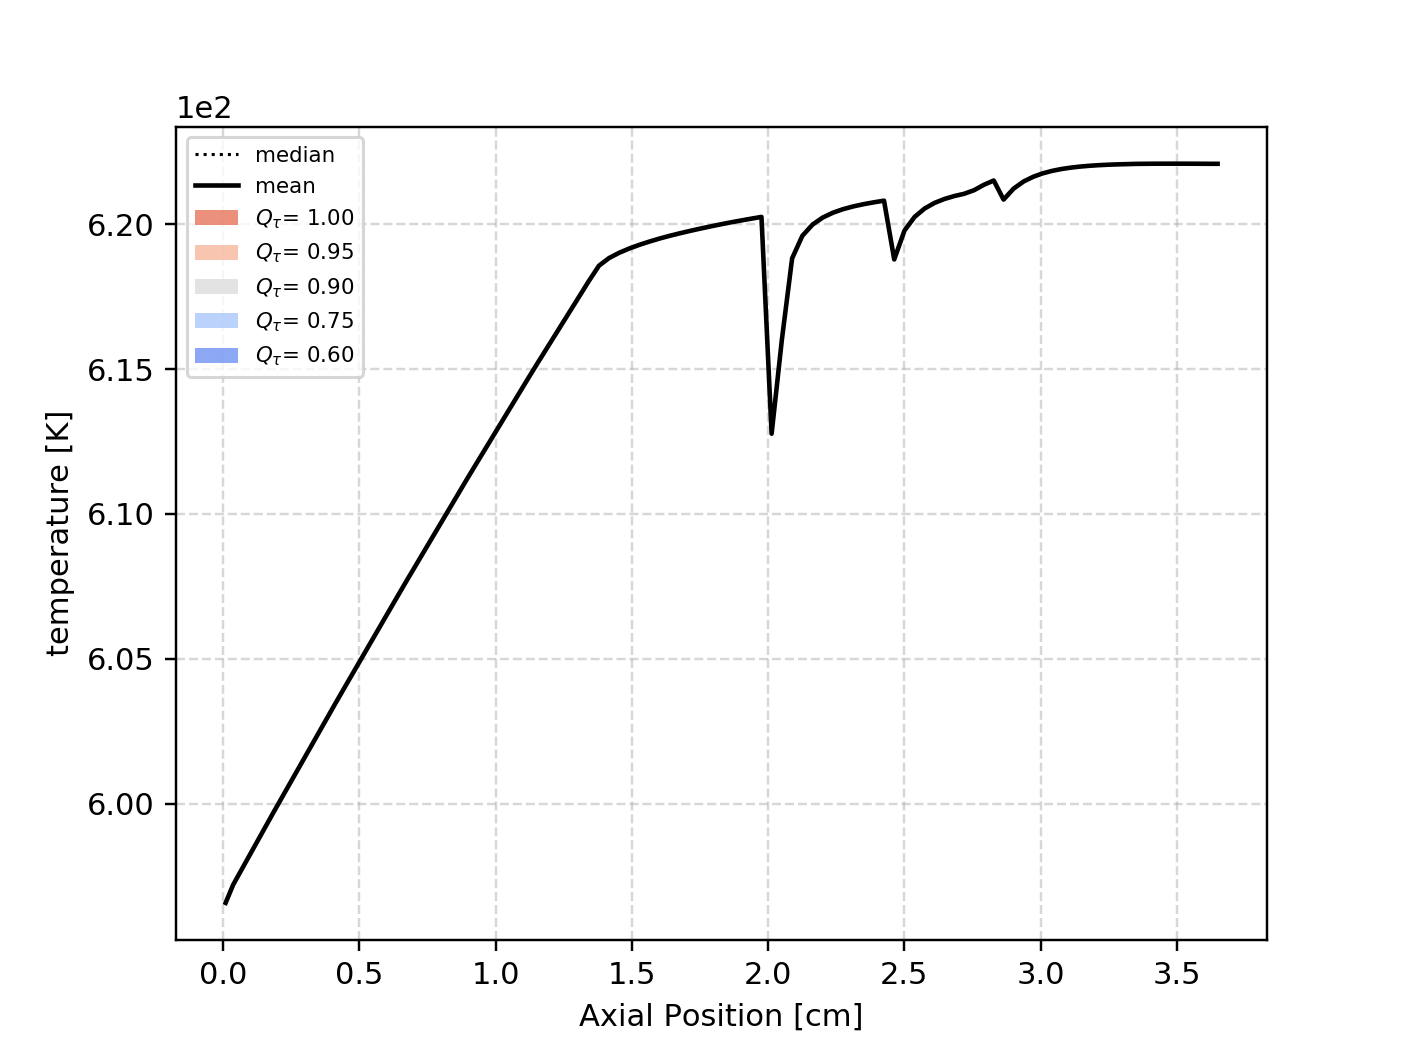
\includegraphics[width=0.53\linewidth]{figs/synth/ctf_asm0_z_twall} }}\hspace*{-1.0em}%
    \subfloat[2-D rod map of CTF result.]{{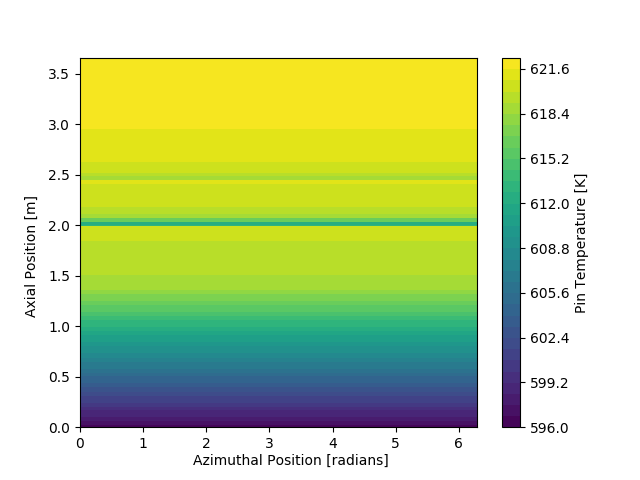
\includegraphics[width=0.53\linewidth]{figs/synth/ctf_pin_h5_temperature} }}%
    \caption[Single pin CTF baseline temperature result.  160\% nominal power conditions.]{Single pin CTF baseline temperature result.  160\% nominal power conditions.}%
    \label{fig:ctf_twall_orig}%
\end{figure}

\begin{figure}[H]%
    \centering
    \subfloat[Axial CTF cladding surface TKE result.]{{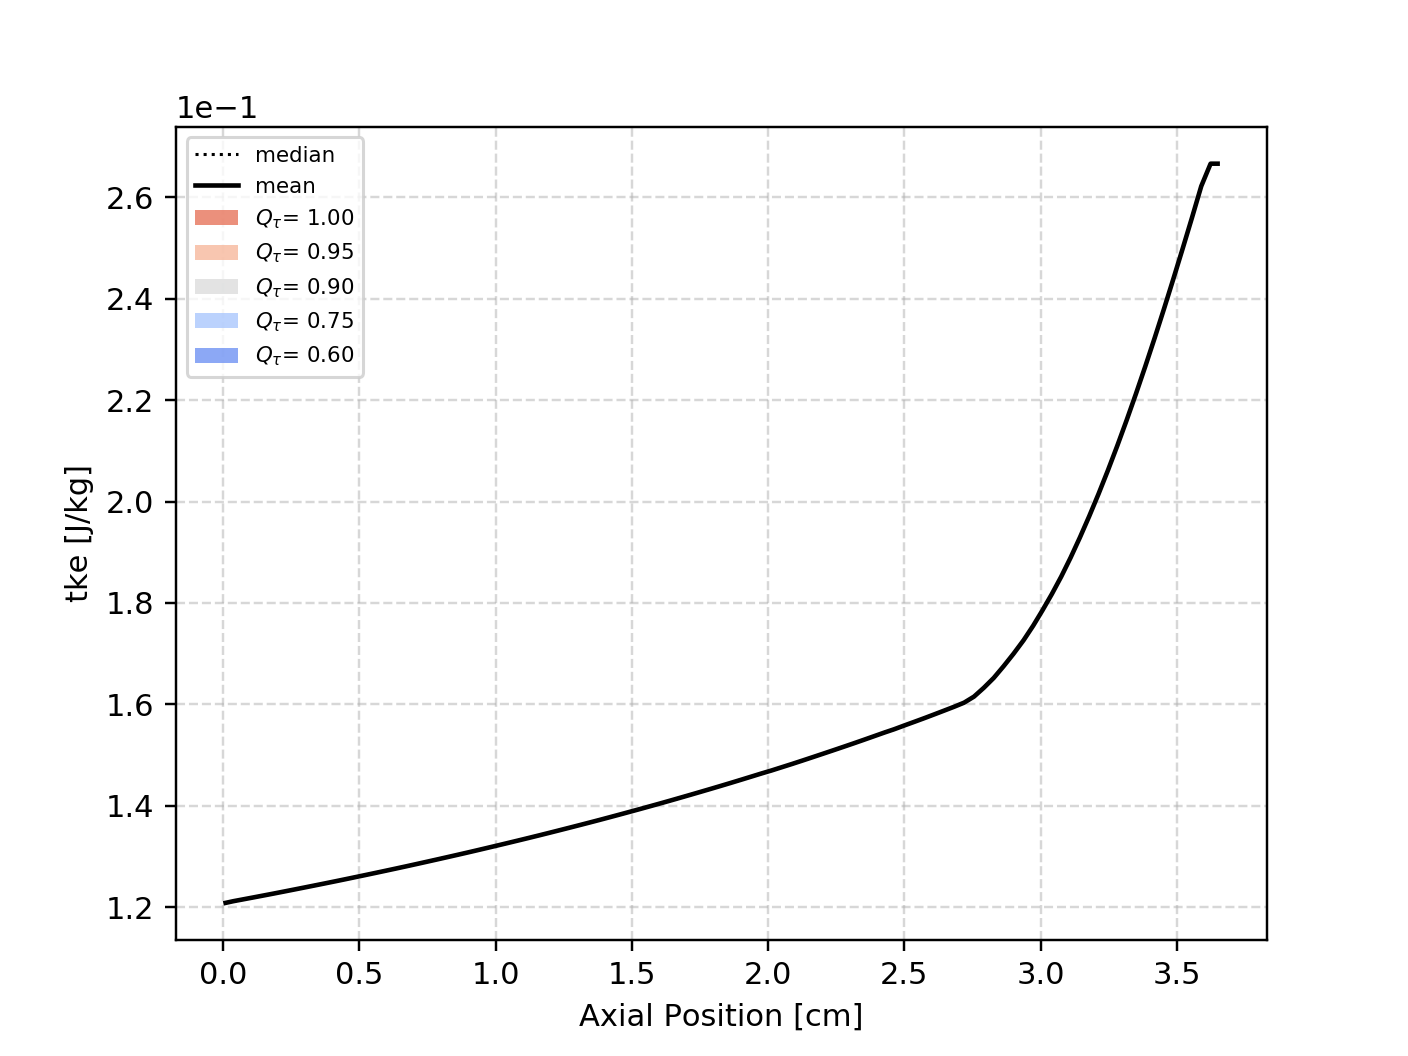
\includegraphics[width=0.53\linewidth]{figs/synth/ctf_asm0_z_tke} }}\hspace*{-1.0em}%
    \subfloat[2-D rod map of CTF result.]{{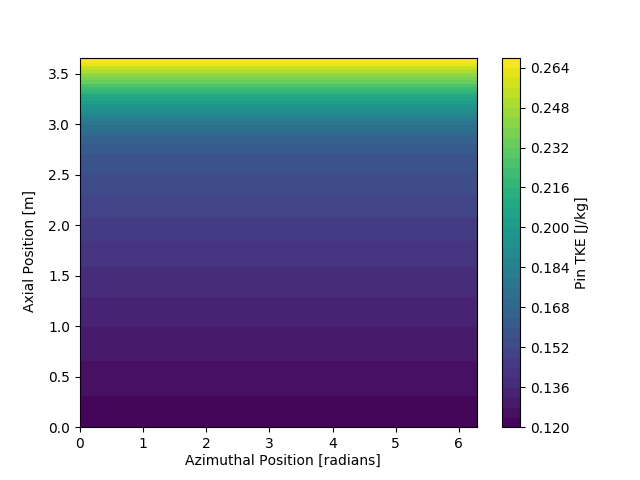
\includegraphics[width=0.53\linewidth]{figs/synth/ctf_pin_h5_tke} }}%
    \caption[Single pin CTF baseline TKE result.  160\% nominal power conditions.]{Single pin CTF baseline TKE result.  160\% nominal power conditions.}%
    \label{fig:ctf_tke_orig}%
\end{figure}


The boundary heat flux was uniform at $85.86 [W/cm^2]$ which corresponds to approximately 160\% nominal PWR power conditions.

Next synthetic noise was generated using copula and marginal distribution settings provided in table \ref{tab:synth_settings}. %The complete synthetic data generation input deck for this case along with references to the code are provided in appendix \ref{chap:app_c}.

\begin{table}[h]
    \begin{center}
        \caption{Per-span synthetic data generation settings.}
        \begin{tabular}{|l|l|l|l|l|}
            \hline
            \bf Span 1 & Node & $z$ & Copula Settings  & Margin Settings \\
            \hline
            $N$: 8000  & 1  & 0.0 & $\Theta_c:$ Gaussian, $\theta_c:-0.6$ &  $T\sim\beta(5.0, 5.0)$,$k\sim\mathcal{N}(0, 0.001)$ \\
                   & 2  & 2.0 & $\Theta_c:$ Gaussian, $\theta_c:-0.6$ &  $T\sim\beta(5.0, 5.0)$, $k\sim\mathcal{N}(0, 0.001)$   \\
            \hline \hline
            \bf Span 2 & Node & $z$ & Copula Settings  & Margin Settings \\
            \hline
             $N$: 8000 & 1  & 2.0 & $\Theta_c:$ Clayton-90, $\theta_c: 2.0$ &  $T\sim\beta(5.0, 2.7)$, $k\sim\beta(1.75, 5.0)$ \\
            & 2  & 2.4 & $\Theta_c:$ Frank-90, $\theta_c: 8.0$ &  $T\sim\beta(5.0, 1.5)$, $k\sim\beta(1.75, 5.0)$   \\
            \hline \hline
            \bf Span 3 & Node & $z$ & Copula Settings  & Margin Settings \\
            \hline
             $N$: 8000 & 1  & 2.4 & $\Theta_c:$ Clayton-90, $\theta_c: 2.0$ &  $T\sim\beta(5.0, 2.7)$, $k\sim\beta(1.75, 5.0)$ \\
            & 2  & 2.8 & $\Theta_c:$ Frank-90, $\theta_c: 8.0$ &  $T\sim\beta(5.0, 1.5)$, $k\sim\beta(1.75, 5.0)$   \\
            \hline \hline
            \bf Span 4 & Node & $z$ & Copula Settings  & Margin Settings \\
            \hline
            $N$: 8000 & 1  & 2.8 & $\Theta_c:$ Clayton-90, $\theta_c: 2.0$ &  $T\sim\beta(5.0, 2.7)$, $k\sim\beta(1.75, 5.0)$ \\
            & 2  & 3.6 & $\Theta_c:$ Frank-90, $\theta_c: 8.0$ &  $T\sim \beta(5.0, 1.5)$, $k\sim\beta(1.75, 5.0)$   \\
            \hline
        \end{tabular}
        \label{tab:synth_settings}
    \end{center}
\end{table}

Samples are drawn with probability proportional to the inverse distance to the nearest specified node.
Let the subscript $(\cdot)_u$ denote the location of the upstream span and $(\cdot)_d$ denote the downstream grid. $d_{u_j}$ and  $d_{d_j}$ denote the distance from the centroid of the CTF face to the nearest upstream and downstream copula nodes respectively.

The mixture joint density model in any given CTF face is specified by equation \ref{eq:dist_weighted_synth}.
\begin{equation}
    h_j = \left( \frac{d_{u_j}}{d_{d} + d_{u}} \right) h_u +
    \left( \frac{d_{d_j}}{d_{d} + d_{u}} \right) h_d
    \label{eq:dist_weighted_synth}
\end{equation}
Where $h_u$ and $h_d$ are the upstream and downstream joint density models respectively with parameters specified in table \ref{tab:synth_settings}.
For simplicity, two copula nodes were specified per span though more are possible for a finer grained control over the marginal and copula distributions.    The copula nodes were located at the span extrema. This node specification pattern allows the synthetic data to mimic the expected sharp change in copula and marginal distributions when moving across spacer grids as seen in the raw CFD data presented in section% \ref{sec:preprocessing} in figure \ref{fig:copula_predicted}.

The copula models were sampled in each span, the original CTF result was augmented with the synthetically generated noise in accordance with equation \ref{eq:synth_aug_discrete}.

\begin{figure}[H]%
    \centering
    \subfloat[Spatial axial augmented CTF result.]{{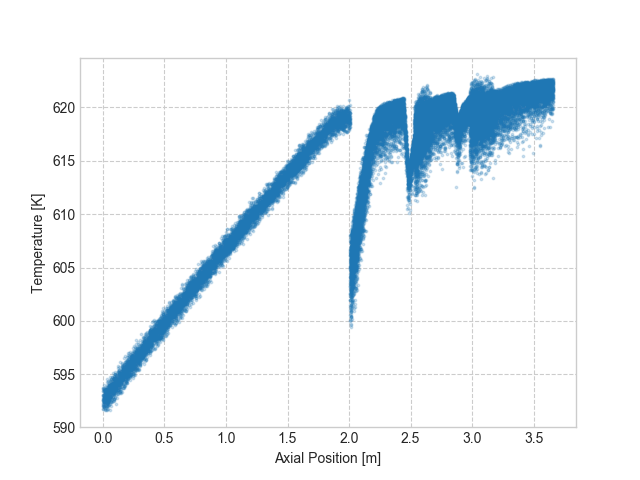
\includegraphics[width=0.53\linewidth]{figs/synth/pinH5TempOut} }}\hspace*{-1.0em}%
    \subfloat[2-D rod map of synthetically augmented CTF result.]{{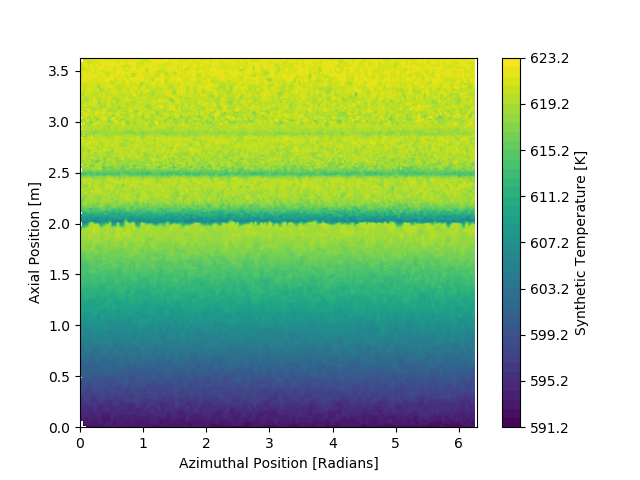
\includegraphics[width=0.53\linewidth]{figs/synth/cfd_pin_temperature} }}%
    \caption[Augmented CFD result.]{Augmented CTF temperature result.}%
    \label{fig:ctf_twall_aug}%
\end{figure}

\begin{figure}[H]%
    \centering
    \subfloat[Spatial axial augmented CTF result.]{{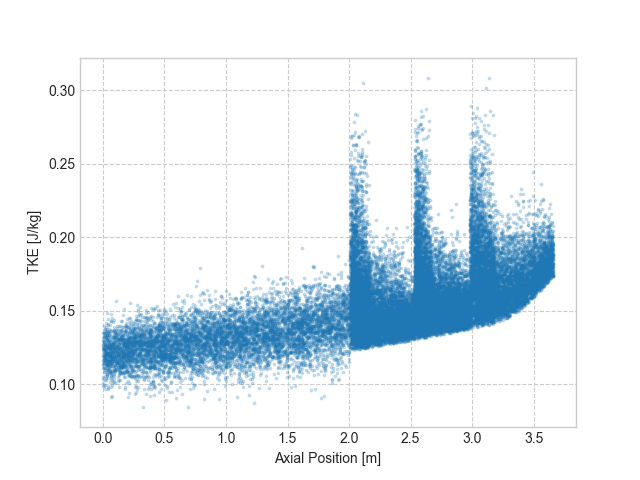
\includegraphics[width=0.53\linewidth]{figs/synth/pinH5TkeOut} }}\hspace*{-1.0em}%
    \subfloat[2-D rod map of synthetically augmented CTF result.]{{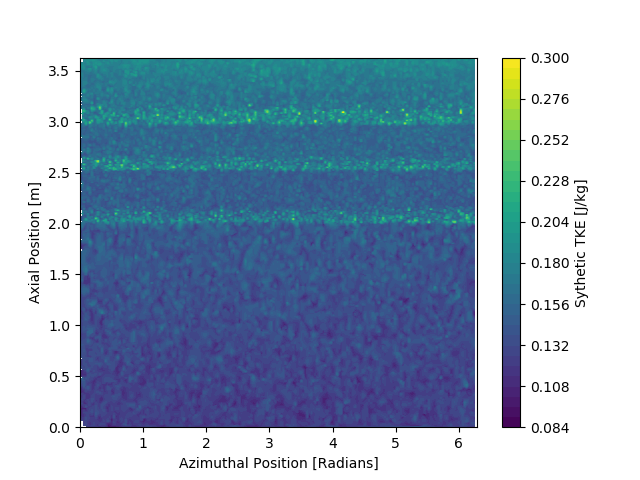
\includegraphics[width=0.53\linewidth]{figs/synth/cfd_pin_tke} }}%
    \caption[Augmented CFD TKE result.]{Augmented CTF TKE result.}%
    \label{fig:ctf_tke_aug}%
\end{figure}

The augmented surface temperature and turbulent kinetic energy fields shown in figures \ref{fig:ctf_twall_aug} and \ref{fig:ctf_tke_aug} may be compared against the original CTF results provided in figures \ref{fig:ctf_twall_orig} and \ref{fig:ctf_tke_orig} respectively to qualitatively understand the fine scale surface variations introduced by the synthetic data model.  No azimuthal variations are present in the augmented fields which would be present if a physics based model, such as CFD, were used.  Additionally, no spatial autocorrelation in the temperature and TKE cladding surface fields are included in the synthetic data.  Spatial autocorrelation could be captured with a kriging model in the future, however, the one dimensional nature of the crud simulation code used in this work dictates that the fine scale spatial detail in the surface fields are irrelevant when computing surface-integrated crud quantities.


\subsection{Single Pin Reconstruction}

The rod surface is subdivided into CTF faces before fitting and reconstructing the synthetic data.  The location and extent of the CTF faces on the rod surface may be determined from a CTF output file.  

In each face the empirical quantile distributions of temperature, turbulent kinetic energy, and boundary heat flux distributions were computed.  The number of quantiles used to construct the empirical quantile distributions was set at 20 and a uniform spacing of quantiles was used.  Copula were fit to the synthetic data based on maximum likelihood and the Akaike information criterion (AIC) in each CTF face.  The maximum likelihood estimation procedure for copula parameters is described in section %\ref{sec:fitting_copula} and the AIC may be computed from equation \ref{eq:cop_aic}.

For the synthetic single pin data the hi2lo predicted fractional surface area above a saturation temperature threshold ($T_{sat}=618.1[K]$) in each CTF face is shown in figure \ref{fig:frac_a}.

\begin{figure}[H]%
    \captionsetup[subfigure]{justification=centering}
    \centering
    \subfloat[][CTF predicted fractional area of each CTF \\ face above the saturation point.]{{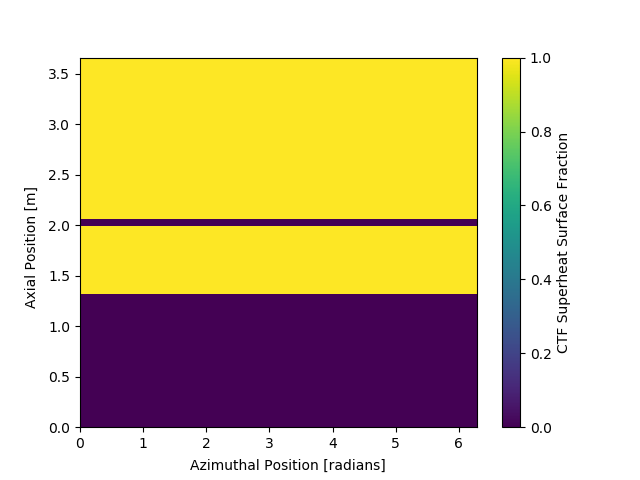
\includegraphics[width=0.53\linewidth]{figs/synth/hi2lo/ctf_pin_t_threshold} }}\hspace*{-1.0em}%
    \subfloat[][Hi2lo predicted fractional area of each \\ CTF face above the saturation point.]{{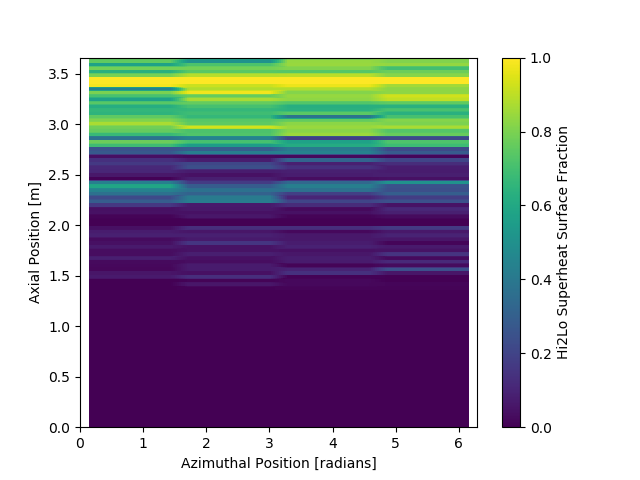
\includegraphics[width=0.53\linewidth]{figs/synth/hi2lo/hi2lo_pin_t_threshold} }}%
    \caption{Fraction of each CTF face above the saturation point predicted by CTF (a) and the hi2lo model (b).}%
    \label{fig:frac_a}%
\end{figure}

Provided that crud growth exhibits a temperature thresholding behavior about the saturation point it is important to predict the fractional area of the rod surface which exists above this critical temperature.  This can be performed by evaluating equation %\ref{eq:pr_thresh} in each CTF face. 
Figure \ref{fig:frac_a} shows a substantial difference in the fractional area predicted above the saturation point in each CTF face when utilizing the hi2lo model rather than the predictions generated from a CTF computation alone.  The more significant the thresholding behavior of crud growth, the more important it becomes to accurately compute areas of the rod surface in excess of the saturation point.

Figure \ref{fig:patchscatter} examines the surface frequency distributions of temperature, crud boron mass and TKE for the CTF patch denoted by the red box in figure \ref{fig:hi2lo_tke_t}.  A marked change in behavior of the crud boron mass vs cladding surface temperature scatter plot is exhibited at approximately $ 619[K]$.  For samples which fell at or below this temperature, little crud was grown and thus the deposited crud boron mass is small.  Past this temperature threshold, there is an approximately linear relationship between the surface temperature and the crud deposition rate.  

An additional feature of note in figure  \ref{fig:patchscatter} is the asymmetric dispersion of the TKE vs. surface temperature scatter plot.  The dependence structure exhibits tighter coupling between these two fields at lower TKE values and less correlation at higher TKE.  This behavior was imposed by specifying a Clayton copula in this location on the rod surface with the copula parameters given in table \ref{tab:synth_settings}.  The ability of the copula fitting routines to correctly preserve this skewed dependence structure is demonstrated in the figure and could not be achieved with multivariate Gaussian models.

\begin{figure}[H]
    \centering
    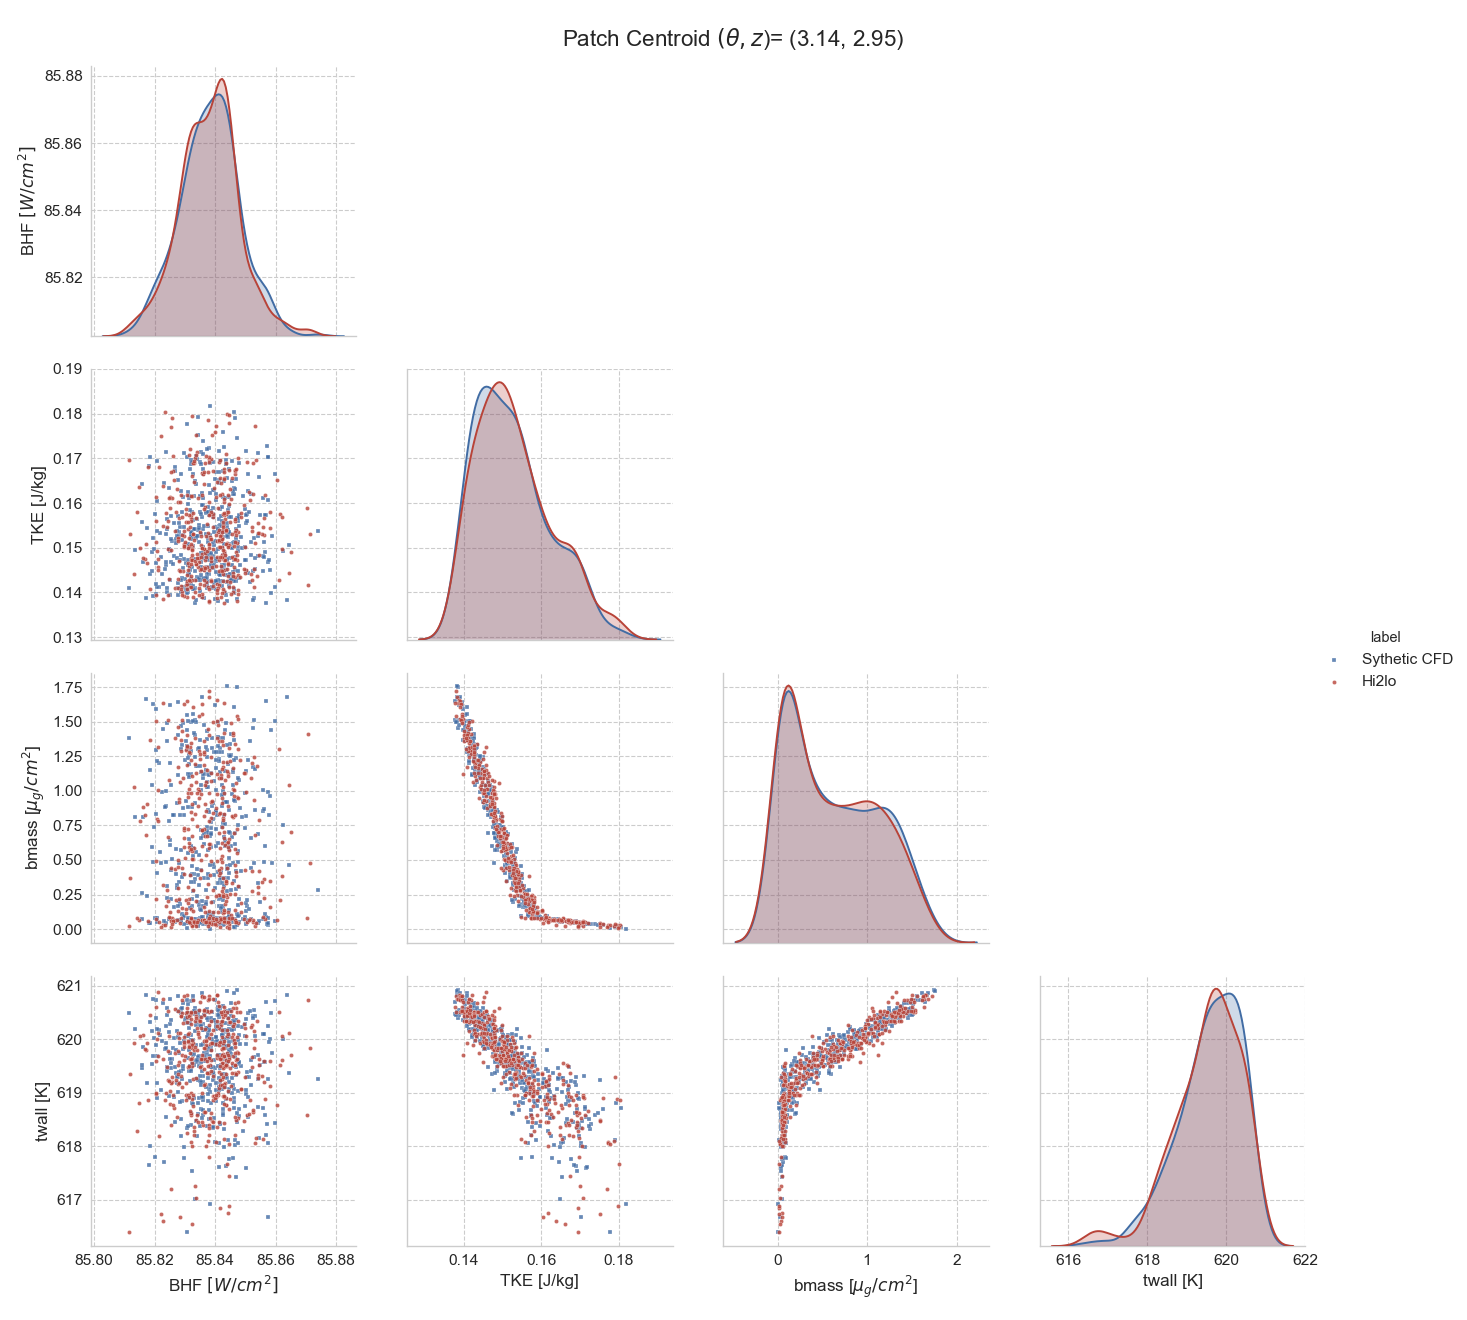
\includegraphics[width=0.99\linewidth]{figs/synth/patch_scatter_0_4_0_6}
    \caption[Single patch synthetic CFD data vs hi2lo sampled data.]{Single patch synthetic data vs hi2lo sampled data from patch centered on the rod at (3.14 $[rad]$, 2.85 $[m]$) at 300$[days]$.  The location of this patch is outlined in red in figure \ref{fig:hi2lo_tke_t}(b).}
    \label{fig:patchscatter}
\end{figure}

\begin{figure}[H]%
    \captionsetup[subfigure]{justification=centering}
    \centering
    \subfloat[Hi2lo temperature reconstruction.]{{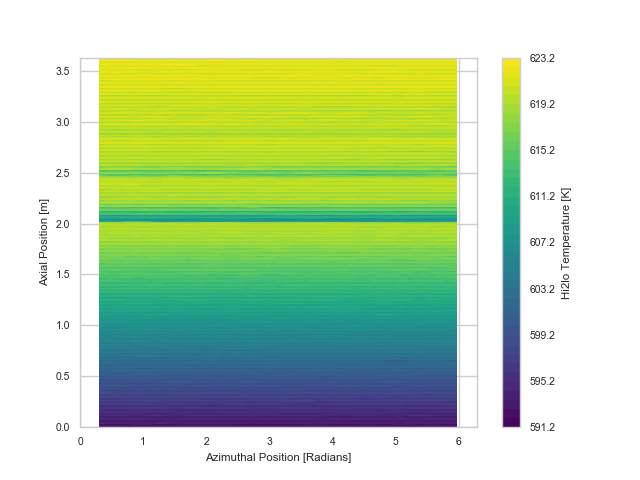
\includegraphics[width=0.58\linewidth]{figs/synth/best_fit/struct_pin_twall} }}\hspace*{-3.1em}%
    \subfloat[Hi2lo TKE reconstruction.]{{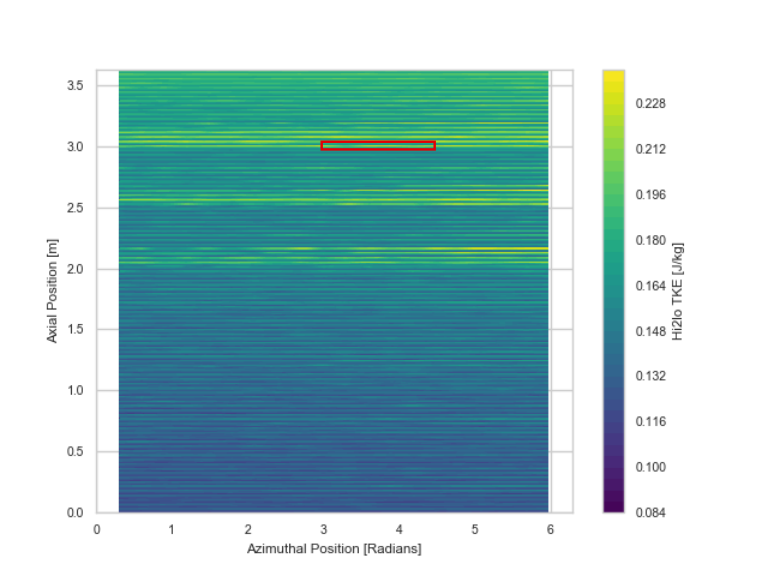
\includegraphics[width=0.58\linewidth]{figs/synth/best_fit/struct_pin_tke_marked} }}%
    \caption[Hi2lo reconstruction of 2-D surface temperature and TKE fields from synthetic CFD data source. ]{Hi2lo reconstruction of 2-D surface temperature and TKE fields from synthetic CFD data source. No azimuthal variation is observed in this quarter symmetric case. }%
    \label{fig:hi2lo_tke_t}%
\end{figure}


After samples are independently drawn in each CTF face the temperature, TKE, and boundary heat flux samples were passed to a crud simulation packages as the cladding-side boundary conditions.  The CTF bulk fluid properties were used as the coolant-side boundary conditions.  The crud simulation was stepped forward for 300 days with a resample step size of $\Delta t_s =50$ days.  400 samples per CTF face were drawn at each resampling event. The resultant crud distribution at 300 days is given in figure \ref{fig:hi2lopincmass}.  Good agreement between the hi2lo predictions and the target synthetic data for the axial crud, temperature, and TKE distributions is exhibited.

\begin{figure}[H]%
    \captionsetup[subfigure]{justification=centering}
    \centering
    \subfloat[Hi2lo axial crud thickness.]{{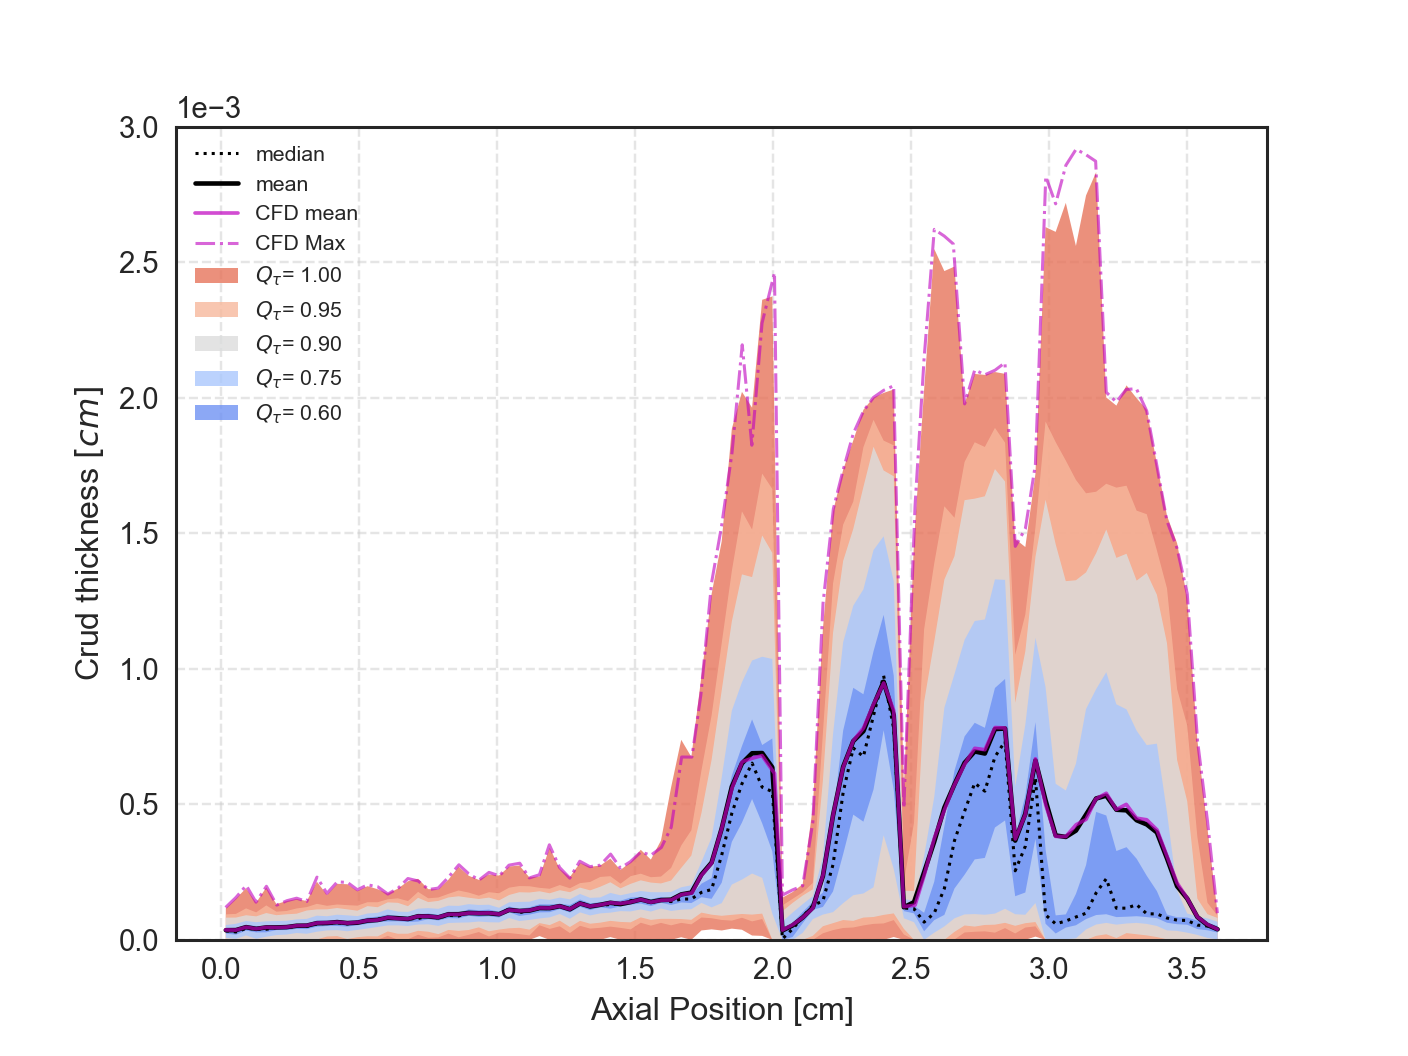
\includegraphics[width=0.53\linewidth]{figs/synth/best_fit/struct_pin_z_cthick300} }}\hspace*{-1.0em}%
    \subfloat[Hi2lo axial crud mass desnity.]{{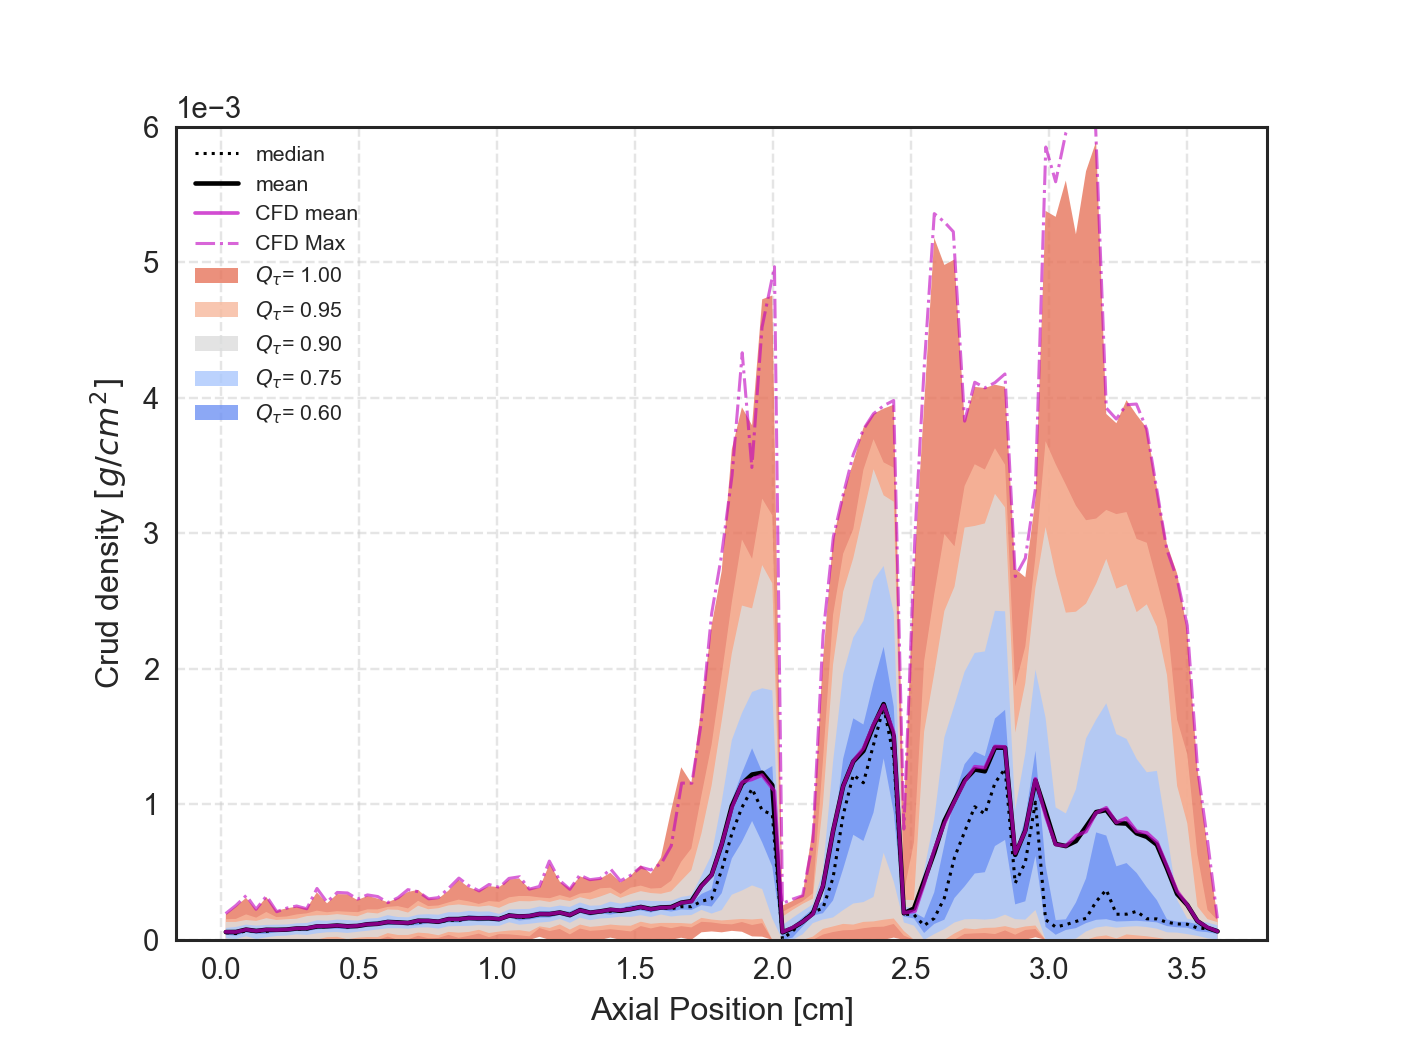
\includegraphics[width=0.53\linewidth]{figs/synth/best_fit/struct_pin_z_cmass_300} }}%
    \caption[Hi2lo axial crud results compared to synthetic CFD/crud results at 300 days simulation time.]{Hi2lo axial crud results compared to synthetic CFD/crud results at 300 days simulation time.  The CFD/crud result is shown in purple.}%
    \label{fig:hi2lopincmass}%
\end{figure}


Table \ref{tab:crud_totals_2} summarizes the hi2lo crud predictions for the synthetic single pin data set.  Good agreement is seen for the rod-integrated crud results.  Again, the hi2lo model was not used in a predictive manner and this represents a best case scenario in which the copula and marginal distribution parameters were directly estimated from the known (synthetic) CFD and CTF data sets.

\begin{table}[h]
    \begin{center}
        \caption[Crud totals for synthetic and hi2lo models.]{Single pin crud totals at 300 days.}
        \begin{tabular}[h]{|l | l | l |}
            \hline
            Copula, $\Theta_c$ & Crud Boron Total: $C_B$ & Crud Mass Total: $C_m$ \\
            \hline  \hline
            Synthetic CFD &  2.79049E-4 $[g]$ & 5.34151E-1 $[g]$ \\
            Hi2lo Reconstruction &  2.78012E-4  $[g]$ & 5.32146E-1 $[g]$ \\
            \hline
            Rel Diff &  0.374 $[\%]$ & 0.377 $[\%]$ \\
            \hline
        \end{tabular}
        \label{tab:crud_totals_2}
    \end{center}
\end{table}



\subsubsection{Crud Copula Parameter Sensitivity}
\label{sec:crud_copula_sensi}

Here the sensitivity of the crud result to the copula parameters is investigated.  Both the impact of the rank correlation coefficient, Kendall's $\tau$, and the Archimedean copula family are investigated.  The sensitivity results generated for the CTF face centered at $\{3.14[rad], 2.95[m]\}$ are shown in figure \ref{fig:patchcrudfit80}.  There is noise present in the crud predictions due to the Monte Carlo integration of equation %\ref{eq:expected_crud} over the patch. 
In this instance 2500 samples were used in the computation of the integral to reduce the magnitude of this noise.  The crud is relatively insensitive to the choice of copula family, but the rank correlation coefficient is shown to have a significant influence on crud growth with an average boron deposition sensitivity of $\frac{\partial C_b}{\partial \rho_\tau} =$ -1.086e-7 $[g/cm^2/\tau]$ for this particular patch.  Accurately predicting Kendall's $\tau$ provided local core conditions is important.
\index{Copula!Crud Sensitivity}

\begin{figure}[H]
    \centering
    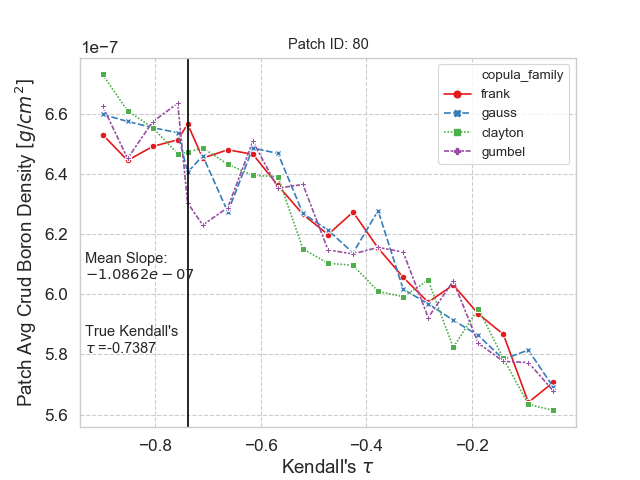
\includegraphics[width=0.8\linewidth]{figs/synth/patch_crud_fit_80}
    \caption{Single CTF face crud sensitivity to copula parameters.}
    \label{fig:patchcrudfit80}
\end{figure}

Next, two full single pin scenarios were considered. In the first scenario, shown in figure \ref{fig:crud_copula_fam_sensi}a, the best-fit copula on each patch as determined by the AIC metric is applied on each CTF face.  The second pin scenario enforces that a Gaussian copula model is used on every CTF face.  The crud results from these scenarios were then compared.  The data shows the choice of copula (between Gaussian, Frank, and Clayton) has a small overall impact on the total integrated rod boron mass.   The total integrated crud mass and crud boron mass for these scenarios at 300 days simulation time are given in table \ref{tab:crud_totals_copula}.

\begin{figure}[H]%
    \centering
    \subfloat[Best fit copula via AIC metric used in each CTF face.]{{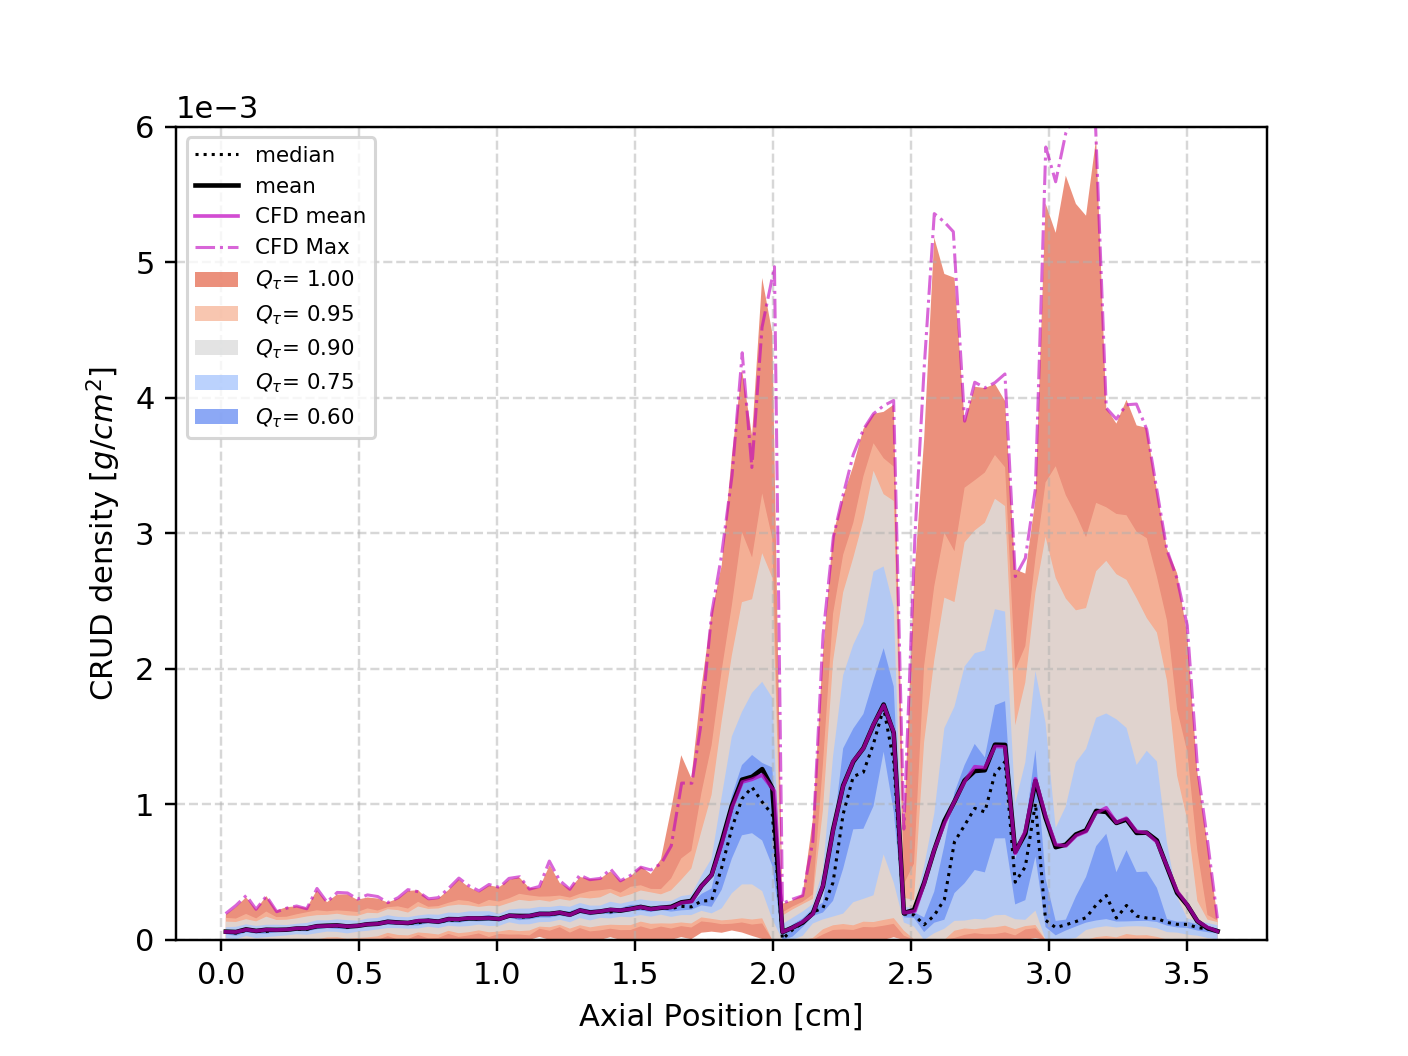
\includegraphics[width=0.53\linewidth]{figs/synth/copula_compare/struct_pin_z_cmass_300_bestfit} }}\hspace*{-1.0em}%
    \subfloat[Gaussian copula used in each CTF face.]{{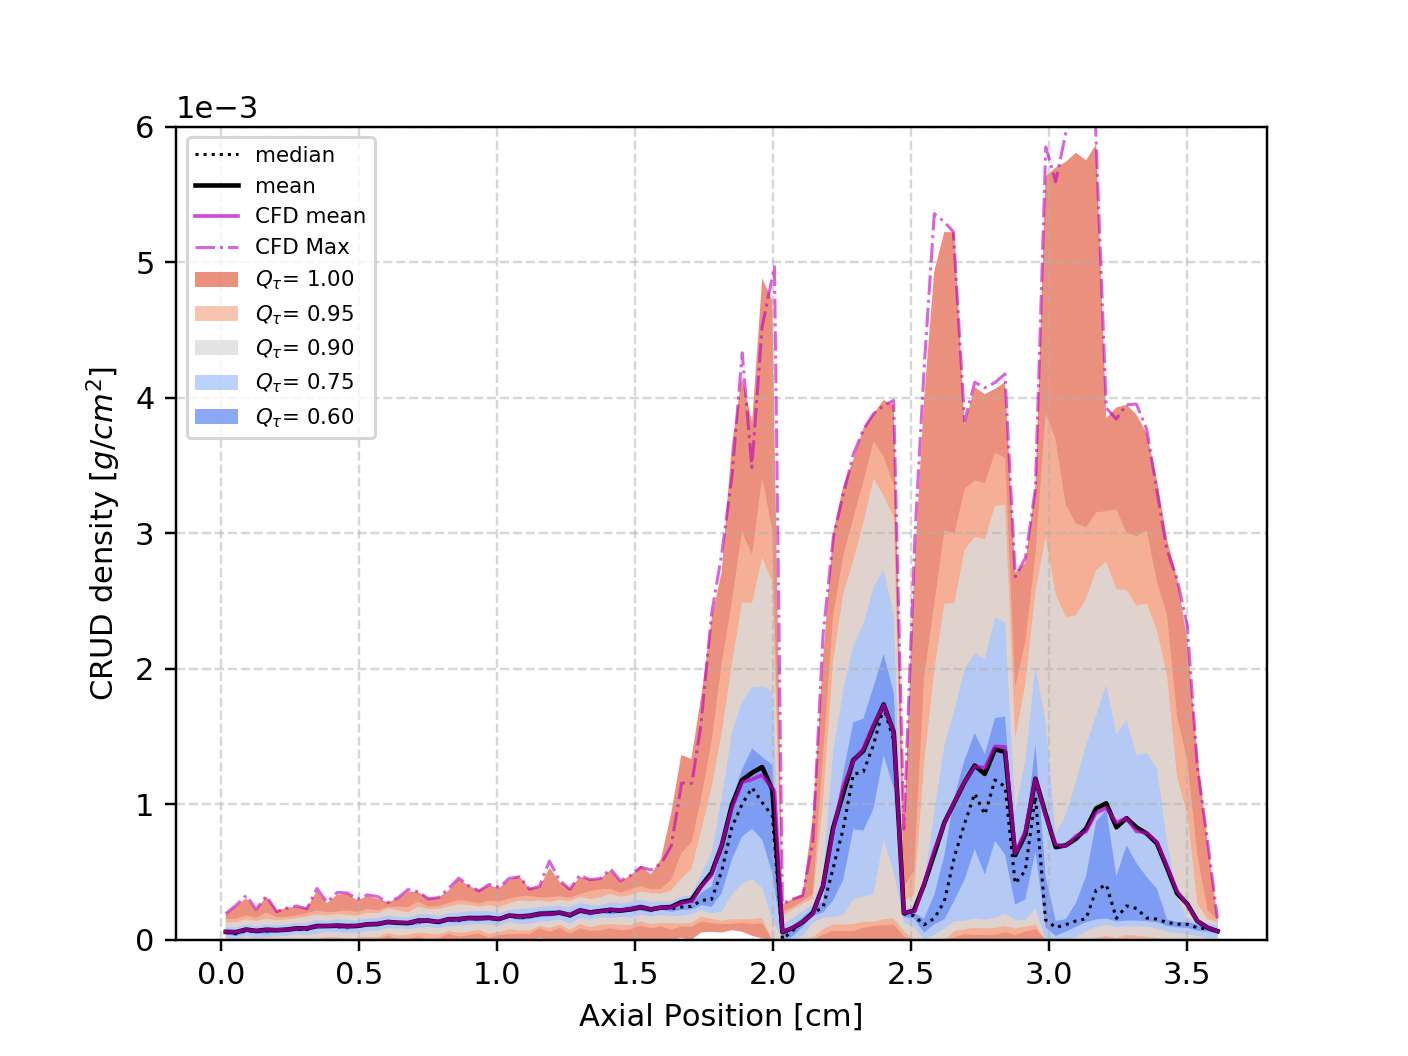
\includegraphics[width=0.53\linewidth]{figs/synth/copula_compare/struct_pin_z_cmass_300_gauss_only} }}%
    \caption[Influence of the choice parameters on the axial crud distribution.]{Influence of the choice parameters on the axial crud distribution.  Synthetic CFD result shown in purple.}%
    \label{fig:crud_copula_fam_sensi}%
\end{figure}


\begin{table}[h]
    \begin{center}
        \caption[Crud totals with different copula assumptions.]{Single pin crud totals at 300 days with different copula assumptions.}
        \begin{tabular}[h]{|l | l | l |}
            \hline
            Copula, $\Theta_c$ & Crud Boron Total: $C_B$ & Crud Mass Total: $C_m$ \\
            \hline  \hline
            Best Fit &  2.78953e-04 $[g]$ & 5.34015e-01 $[g]$ \\
            Gaussian &  2.78301e-04 $[g]$ & 5.32769e-01 $[g]$ \\
            \hline
            Rel Diff &  0.017 $[\%]$ & 0.234 $[\%]$ \\
            \hline
        \end{tabular}
        \label{tab:crud_totals_copula}
    \end{center}
\end{table}

The choice of the copula family, $\Theta_c$, has a negligible impact on the integrated crud results over a pin.  This result reduces the complexity of the hi2lo model by removing the need to predict the correct copula family on each CTF patch in the core. % In section \ref{sec:preprocessing} it is shown that CFD data exhibits a complex relationship between the best fitting copula family and the axial position along the rod.
This relationship proved difficult to model using standard classification techniques, though further testing with a larger quantity of training data is warranted to ascertain if the copula family describing the dependence between the temperature and TKE fields on the rod surface may be accurately predicted given local core conditions.

\subsubsection{Crud Sample Size Study}

The number of samples, $N$, used to estimate the integral given in equation %\ref{eq:mc_expected_crud} is a parameter set at runtime of the hi2lo method. 
Here, it is shown that the integrated crud variance is reduced by increasing the number of samples used per CTF face to estimate the integrated crud quantities of interest.   Furthermore, section \ref{sec:Importance Sampling} demonstrates that improvements in sampling efficiency are possible by way of importance sampling.

Figure \ref{fig:cmprpintotalsviolinnsample} shows the variance of the crud expectation value at 300 days of simulation time computed by the Monte Carlo approximation when using a sample sizes of 100, 400, and $800  [\frac{N}{\mathrm{CTF_{face}}}]$.  80 independent trials were conducted for each sample size to estimate the variance of the pin integrated crud results at 300 days.

To isolate the impact of increasing the sample size on the crud variance, a single 300 day time step was conducted without resampling the underlying density functions during this period.  Importance sampling was not applied in this study.

\begin{figure}[H]
    \centering
    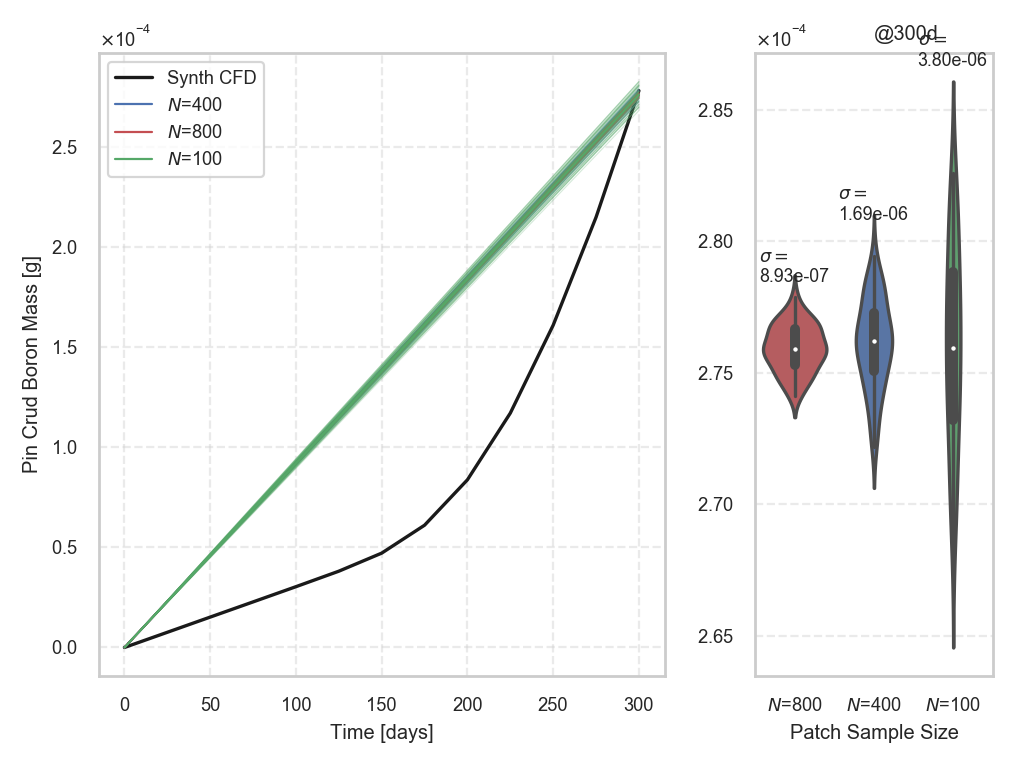
\includegraphics[width=0.8\linewidth]{figs/synth/nsample_study/cmpr_pin_totals_violin_nsample}
    \caption{Effect of sample size on the integrated crud results.}
    \label{fig:cmprpintotalsviolinnsample}
\end{figure}

The standard deviation of the rod integrated crud results at 300 days simulation time are summarized in table \ref{tab:crud_sample_size}.

\begin{table}[h]
	\begin{center}
		\caption[Estimated sensitivity of the pin-integrated crud boron variance to the number of samples used per CTF face.]{Estimated sensitivity of the pin-integrated crud boron variance to the number of samples used per CTF face. Variance estimated using 80 independent trials.}
		\begin{tabular}[h]{| c | C | C |}
			\hline
			N  & Mean Pin Crud Boron Total $[g]$ & Pin Integrated Crud Boron Std. Dev. $[g]$ \\
			\hline  \hline
			100 &  2.78953e-04  & 3.80e-6  \\
			400 &  2.78301e-04  & 1.69e-6  \\
			800 & 2.78411e-04 & 8.93e-7 \\
			\hline
		\end{tabular}
		\label{tab:crud_sample_size}
	\end{center}
\end{table}


\subsubsection{Importance Sampling}
\label{sec:Importance Sampling}

To obtain estimates for the efficiency gain offered by importance sampling to compute the expected crud value by equation %\ref{eq:mc_imp_expected_crud}, a singe patch was studied under synthetic TH data.

Here, the design of the sampling routines and the physics of crud growth is intertwined.  To compute the integral %\ref{eq:expected_crud} efficiently it is favorable to sample the TH distribution in regions which result in relatively large amounts of crud growth. 
To guide the design of the importance distributions the response surface of the crud simulation code is presented in figures \ref{fig:crud_sensi1} to \ref{fig:crud_sensi3}.  Larger surface temperatures result in a higher crud growth rate.  Larger local TKE results in smaller crud growth rates due to the effects of erosion.  Note the relatively small influence of the boundary heat flux on the crud growth rate.  This is an important observation used to justify simplifications made in the joint density model previously provided in equation %\ref{eq:simple_vine_model}.

\begin{figure}[H]%
    \captionsetup[subfigure]{justification=centering}
    \centering
    \subfloat[][Crud boron deposition sensitivity  to \\ temperature with TKE held fixed at $0.05$ {[J/kg]}.]{{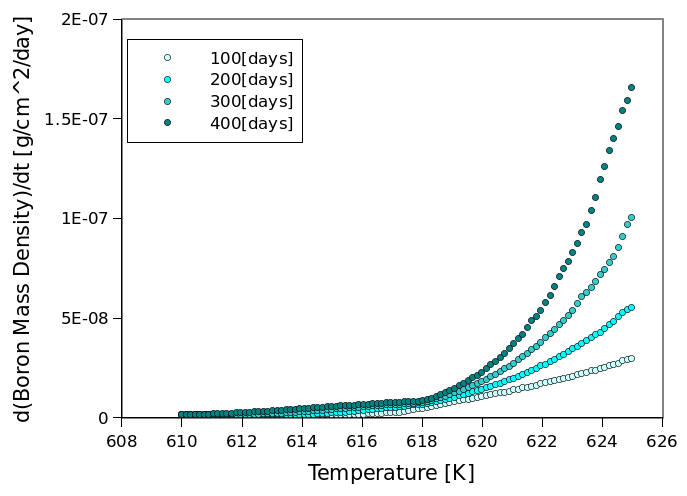
\includegraphics[width=0.51\linewidth]{../proposal/slides/seminar_slides/figs/dboron_dt_t} }}\hspace*{-1.0em}%
    \subfloat[][Crud boron deposition sensitivity to TKE \\ with temperature held fixed at $620$ {[K]}.]{{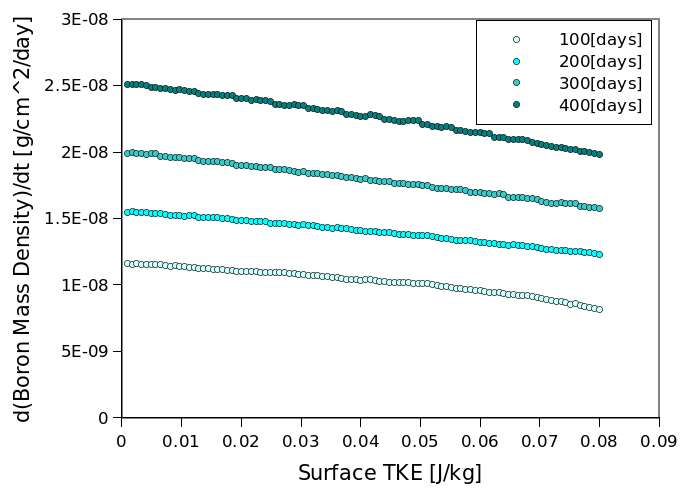
\includegraphics[width=0.51\linewidth]{../proposal/slides/seminar_slides/figs/dboron_dt_tke} }}%
    \caption[Crud marginal response to varying temperature and TKE at different times.]{Crud deposition rate sensitivity to varying temperature and TKE at different times.}%
    \label{fig:crud_sensi1}%
\end{figure}

In figure \ref{fig:crud_sensi1} the crud growth rate response is depicted at 100 day increments.  At temperatures exceeding the saturation temperature ($\approx 618[K]$) a marked change in crud growth rates is exhibited.  When the saturation temperature is exceeded on the rod surface there is a rise in crud deposition rates and the rate at which boron is precipitated inside the crud layer.

\begin{figure}[H]%
    \captionsetup[subfigure]{justification=centering}
    \centering
    \subfloat[][Crud boron deposition sensitivity with \\ $q''=80 {[W/cm^2]}$.]{{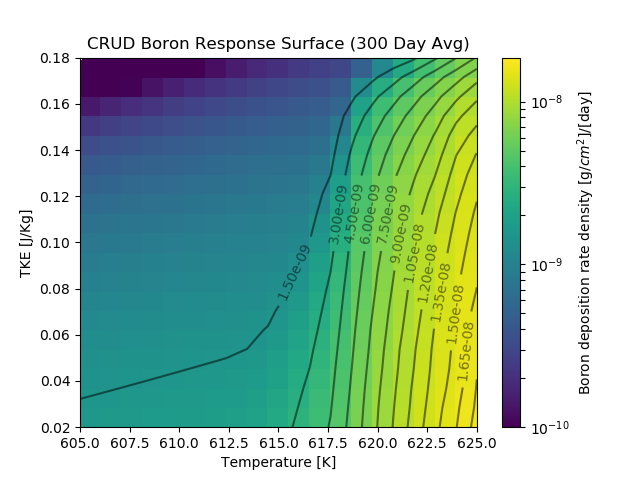
\includegraphics[width=0.53\linewidth]{figs/crud/crud_t_tke_boron_response_80} }}\hspace*{-1.0em}%
    \subfloat[][Crud boron deposition sensitivity \\  $q''=120 {[W/cm^2]}$.]{{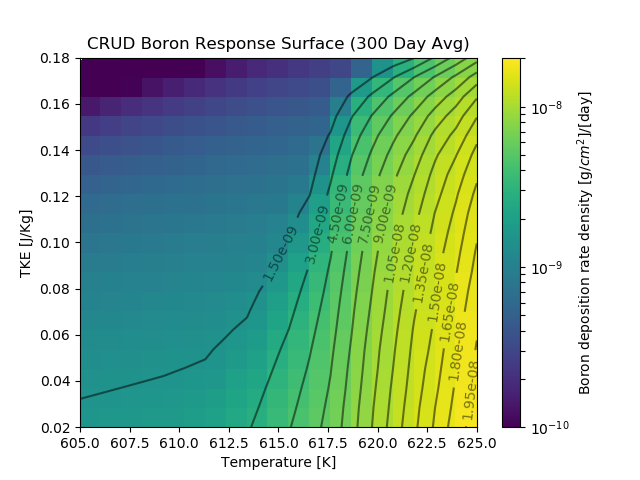
\includegraphics[width=0.53\linewidth]{figs/crud/crud_t_tke_boron_response_120} }}%
    \caption[Crud boron response to varying temperature and TKE.]{Crud boron response surface to varying temperature and TKE. The crud boron deposition rate is relatively insensitive to the boundary heat flux.}%
    \label{fig:crud_sensi2}%
\end{figure}

\begin{figure}[H]%
    \centering
    \subfloat[][Crud mass deposition sensitivity \\ $q''=80 {[W/cm^2]}$.]{{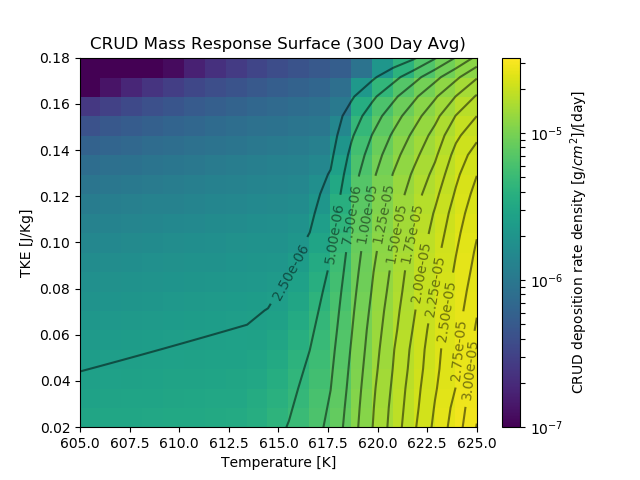
\includegraphics[width=0.53\linewidth]{figs/crud/crud_t_tke_mass_response_bhf_80} }}\hspace*{-1.0em}%
    \subfloat[][Crud mass deposition sensitivity \\ $q''={[120 W/cm^2]}$.]{{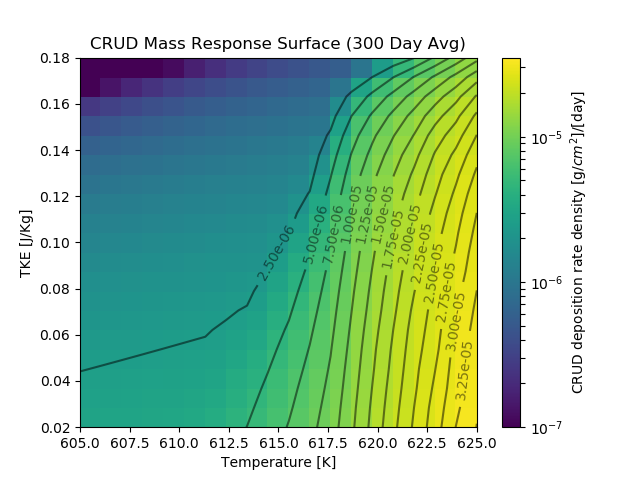
\includegraphics[width=0.53\linewidth]{figs/crud/crud_t_tke_mass_response_bhf_120} }}%
    \caption[Crud mass response surface to varying temperature and TKE.]{Crud mass response surface to varying temperature and TKE. The crud mass deposition rate is relatively insensitive to the boundary heat flux.}%
    \label{fig:crud_sensi3}%
\end{figure}

Though an optimal importance distribution, $\tilde{h}^* $, can be found by equation \ref{eq:optimal_imp},

\begin{equation}
\tilde{h}^* = \mathrm{argmin}_{\tilde{h}}\mathrm{Var} \left[ \frac{\mathcal{G}(x)h(x)}{\tilde{h}(x)} \right] 
\label{eq:optimal_imp}
\end{equation}

the requisite minimization problem is not solved in this work and is left as an avenue for future investigation. It may be shown that the optimal importance distribution follows the form: $\tilde{h}^* \propto |\mathcal{G}(x)|h(x)$, \cite{rubinstein2011}, \cite{mcbook}.

Although the theoretically optimal importance distribution is not achieved in this work, a locally adaptive importance function was adopted based on a distribution mixing approach.  Through the mixture formulation, the importance distributions can be made to depend on the temperature and TKE marginal distributions in a particular CTF face.  The temperature and TKE distributions in each CTF face are mixed with a beta distribution whose parameters are set at runtime of the hi2lo tool.  

The importance  mixture quantile functions are defined in equations \ref{eq:imp_mix_k} and \ref{eq:imp_mix_T}.

\begin{align}
\tilde Q_{j,k} &= \lambda_{0,k} \hat Q_{j,k}  + \lambda_{1,k} Q_{\beta_k}(k; \vartheta_k),  \label{eq:imp_mix_k} \\
\tilde Q_{j,T} &= \lambda_{0,T} \hat Q_{j,T}  + \lambda_{1,T} Q_{\beta_T}(T; \vartheta_T);  \label{eq:imp_mix_T} \\
\sum_i \lambda_i &= 1, \ \ \tilde F_{j,T} = \tilde Q^{-1}_{j,T},\ \  \tilde F_{j,k} = \tilde Q^{-1}_{j,k}
\label{eq:imp_mix_dists}
\end{align}
Where $\tilde Q_{j,T}$ is the quantile function for the proposal temperature distribution in the $j^{th}$ CTF face. $\lambda_i$ are user set mixture weights. Standard Monte Carlo sampling can be recovered by setting $\lambda_{0,k}=1,\ \lambda_{0,T}=1$ and  $\lambda_{1,k}=0,\ \lambda_{1,T}=0$.

Beta distributions, with quantile functions $Q_{\beta_k}$ and $Q_{\beta_T}$,  with proscribed parameters, $\{ \vartheta_k, \vartheta_T \}$, are used in mixture with the original target temperature and TKE density functions to produce a proposal density distribution for each patch.  To provide additional flexibility in the design of proposal density, the mixture weights may be adjusted. By suitably tuning the parameters of the beta distributions and mixture weights, one can target the hot locations of the rod which occur in coincidence with low TKE.  Mixture settings denoted in table %\ref{tab:hi2lo_params} were adopted for this work.
Shown in figure \ref{fig:imp_sample2} with proper tuning of the mixture distribution parameters, the sampling distribution may be skewed towards higher temperatures and lower TKE.

\begin{figure}[H]%
    \centering
    \subfloat[Temperature distributions.]{{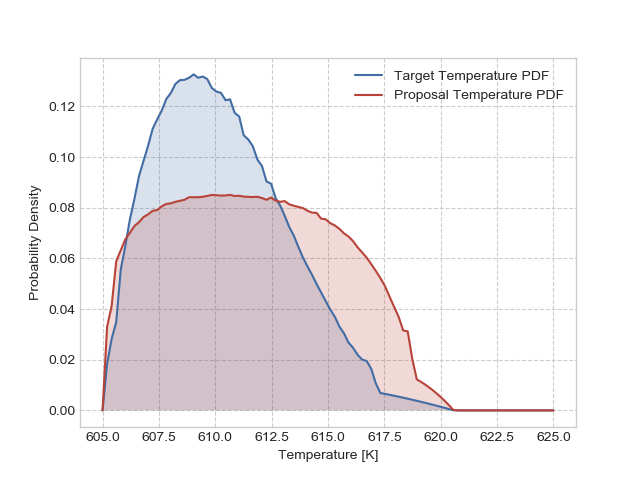
\includegraphics[width=0.53\linewidth]{figs/imp_patch/temperature_importance_marginal_compare} }}\hspace*{-1.0em}%
    \subfloat[TKE distributions.]{{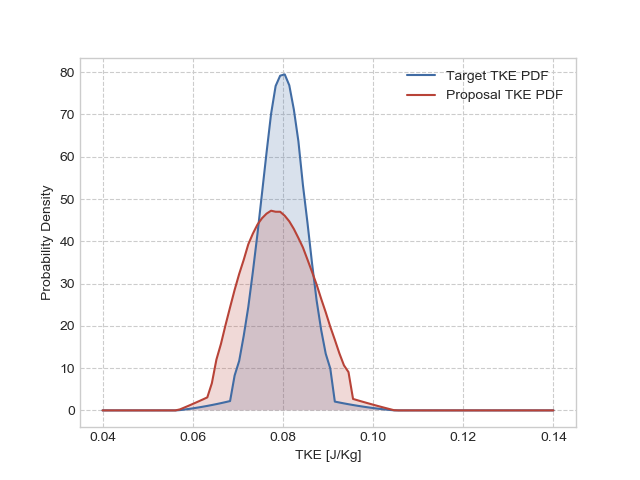
\includegraphics[width=0.53\linewidth]{figs/imp_patch/tke_importance_marginal_compare} }}%
    \caption[Proposal and target density functions used for importance sampling.]{Proposal (red) vs. original (blue) marginal distributions for the (a) surface temperature and (b) TKE.  Generated using importance distribution parameters: $\vartheta_T = \{1, 0.9\}$,  $\vartheta_k = \{1.1, 1.2\}$,  $\lambda_{0,T}=0.6,\ \lambda_{1,T}=0.4$ and $\lambda_{0,k}=0.7,\ \lambda_{1,k}=0.3$.}%
    \label{fig:imp_sample2}%
\end{figure}


\begin{figure}[H]%
    \centering
    \subfloat[Crud boron mass deposition.]{{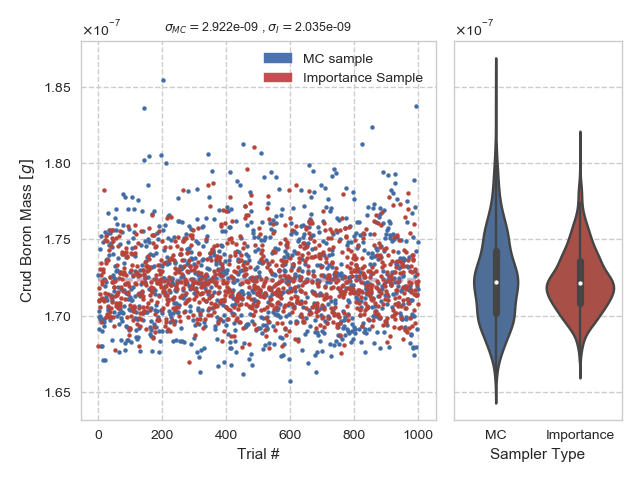
\includegraphics[width=0.53\linewidth]{figs/imp_patch/bmass_sample_violin} }}\hspace*{-1.0em}%
    \subfloat[Crud mass deposition.]{{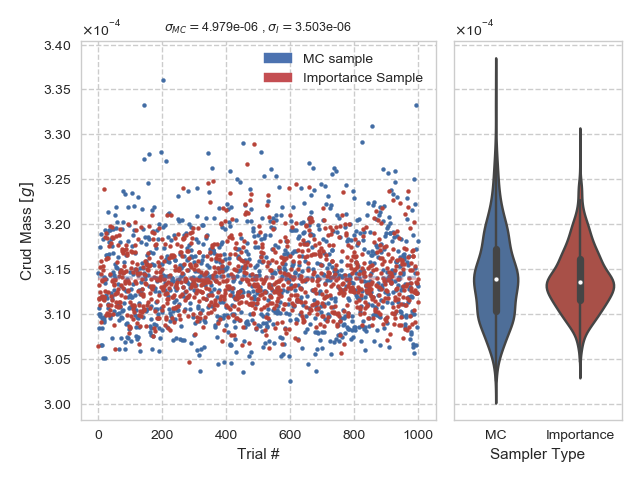
\includegraphics[width=0.53\linewidth]{figs/imp_patch/cmass_sample_violin} }}%
    \caption[Importance sampling results.]{Importance sampling trial results on a single CTF face for (a) crud boron mass deposition and (b) Crud mass deposition at 300 days.  Red denotes importance samples and blue denotes standard Monte Carlo samples.  The sample population variance is shown above the figure for each case and the full sample distributions are given in the margins.}%
    \label{fig:imp_sample1}%
\end{figure}

In figure \ref{fig:importancettkebmassscatter} the relative importance weight is denoted by the size of each point in the scatter plot.  Samples which have a small ratio $(h_i/\tilde h_i)$ appear as small points.  The sample weight is analogous to the rod surface area occupied by the sample.  In comparison, figure \ref{fig:originalttkebmassscatter} shows the same patch using a standard Monte Carlo sampling where each sample has the same weight.  The number of samples drawn in the upper tail of the temperature distribution is greater when importance sampling is applied, though these samples carry expectedly small sample weights.

\begin{figure}[H]
    \centering
    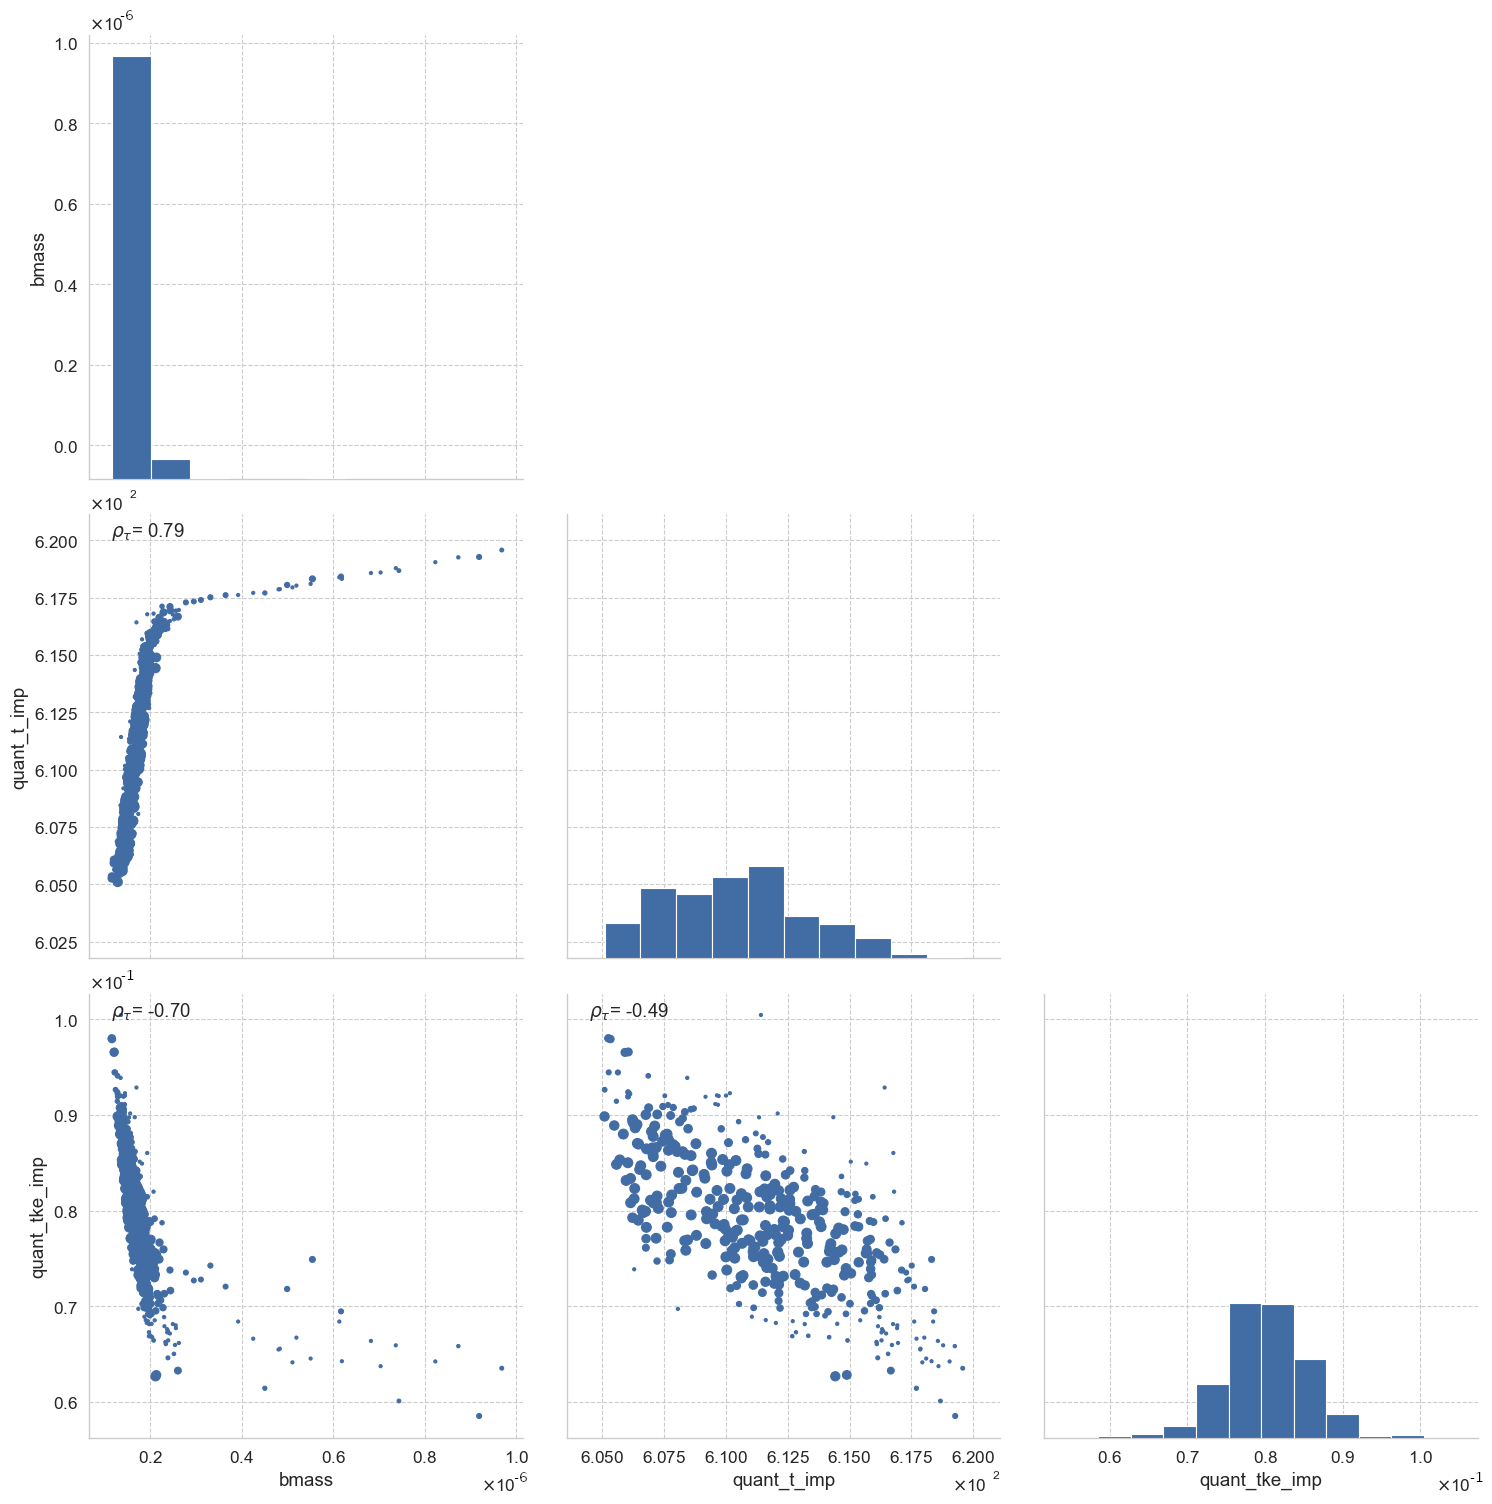
\includegraphics[width=0.99\linewidth]{figs/imp_patch/importance_t_tke_bmass_scatter}
    \caption[Importance sampled single patch crud scatter plot result.]{Importance sampled single patch crud result. Key: \textbf{quant\_t\_imp}: Importance samples from quantile-reconstructed patch temperature $[K]$ distribution with $N_{Q_T}=20$,  \textbf{quant\_tke\_imp}: Importance samples from quantile-reconstructed patch TKE $[J/kg]$ distribution with $N_{Q_k}=20$,  \textbf{bmass}:  Resultant crud boron mass density samples in $[g/cm^2]$. Relative importance weights are denoted by the point size.}
    \label{fig:importancettkebmassscatter}
\end{figure}

\begin{figure}[H]
    \centering
    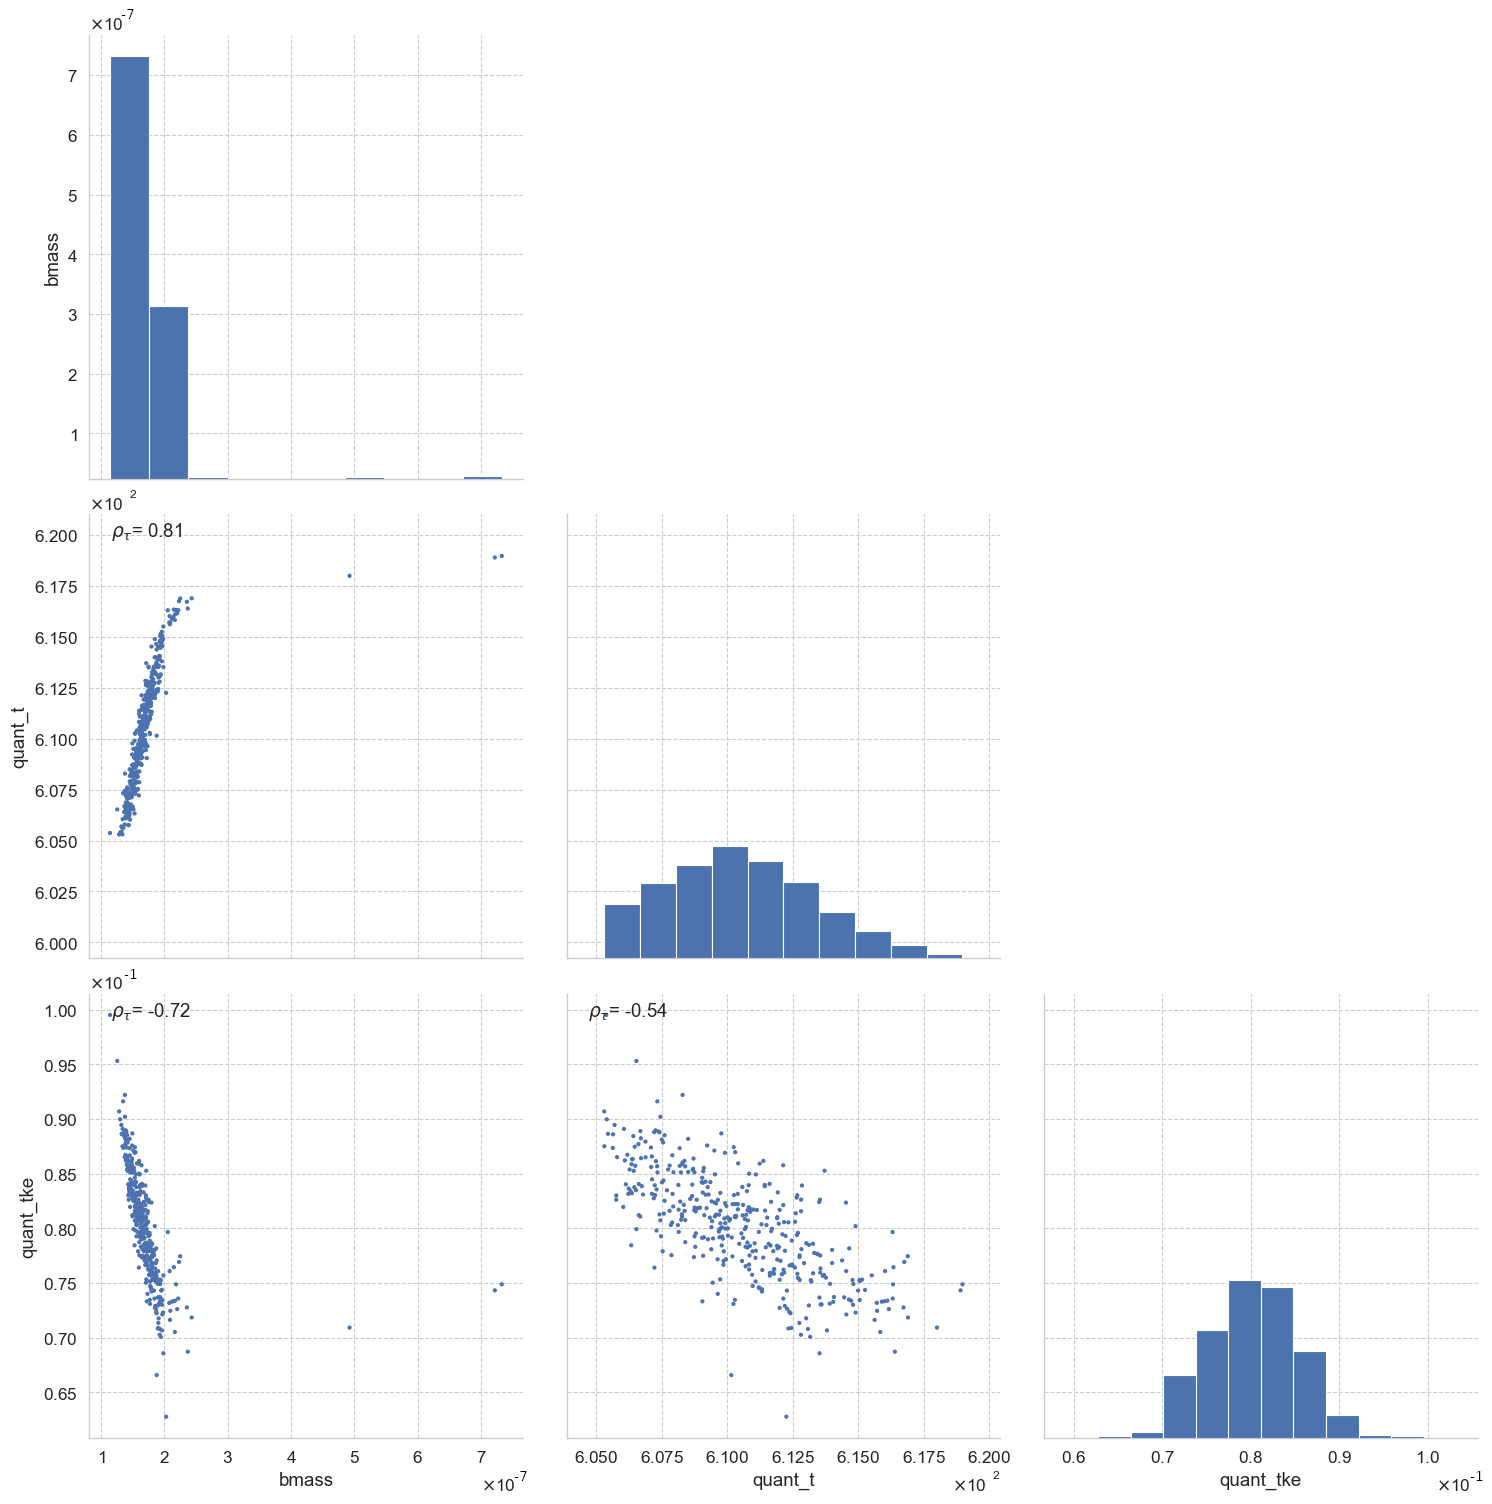
\includegraphics[width=0.99\linewidth]{figs/imp_patch/original_t_tke_bmass_scatter}
    \caption[Standard Monte Carlo sampled patch crud scatter plot result.]{Standard Monte Carlo sampled patch crud result. Key: \textbf{quant\_t}: Samples from quantile-reconstructed patch temperature $[K]$ distribution with $N_{Q_T}=20$,  \textbf{quant\_tke}: Samples from quantile-reconstructed patch TKE $[J/kg]$ distribution with $N_{Q_k}=20$,  \textbf{bmass}: Resultant crud boron mass density samples in $[g/cm^2]$.  }
    \label{fig:originalttkebmassscatter}
\end{figure}
\index{Importance Sampling!Application}

The importance sampling efficiency was estimated by computing the variance ratio:  $\sigma^2_{MC}/\sigma^2_{I}$.  The variance of the patch-integrated crud result for the Monte Carlo and importance sampling schemes are provided in figure \ref{fig:imp_sample1}.  The variance estimates were computed by running 1000 independent trials in which crud was grown on the patch for 300 days.  A total of 100 samples per patch per trial were used.  For the case studied, the application of importance sampling reduced the crud mass and boron mass sample variance by a factor of 2.02. $\frac{\sigma^2_{MC}}{\sigma^2_{I}} \approx (\num{4.979e-6})^2 / (\num{3.503e-6})^2  \approx 2.02$.  The mean crud predictions did not significantly deviate between two sampling schemes indicating that importance sampling does not introduce any bias in the evaluation of the integral in equation %\ref{eq:expected_crud}.

The improvement in performance afforded by importance sampling may be attributed to expending a larger proportion of the total available samples in the upper tail of the temperature distribution as this is a region which strongly contributes to crud growth.  Some samples are necessarily expended in cold regions of the rod surface but occur with less frequency when compared to a standard Monte Carlo sampling routine and the samples are appropriately weighted to avoid biasing the integrated result.


\subsection{Single Pin with Time Stepping}

Stepping the crud simulation forward under the application of hi2lo supplied boundary conditions demands careful treatment of hot spot stationarity assumptions.  The time evolution of the crud simulation on the rod surface is strongly influenced by choices made both in the number of resampling steps taken as well as tunable constants which govern the sample remapping procedure and surface temperature mixing.

\subsubsection{Spatial Remapping with Time Stepping}

The influence of hot-spot stationarity assumptions on the overall integrated crud mass on the rod as a function of time can be seen in figures \ref{fig:cmprpintotals0406} and \ref{fig:cmprpintotalsnoremap}.  When the surface temperature is allowed to randomly mix on each resampling event in each CTF face, the influence of the hot spots are smeared over the surface of the rod which leads to an overall under prediction in the total integrated crud mass.  Reordering the samples in each CTF face by their temperature improves the ability of the hi2lo model to preserve the impact of stationary hot and cold spots on the rod surface.  Good agreement with the original coupled synthetic CFD-Crud simulation data was achieved by tuning the constants introduced in equation %\ref{eq:weighting} to values of $w_T = 0.4$, and of $w_k = 0.6$.  
This weighting seeks to preserve a heuristic thermal-hydraulic metric on the rod surface  where the metric may be interpreted as some linear combination of cladding surface temperature and near-wall TKE.


\begin{figure}[H]
    \centering
    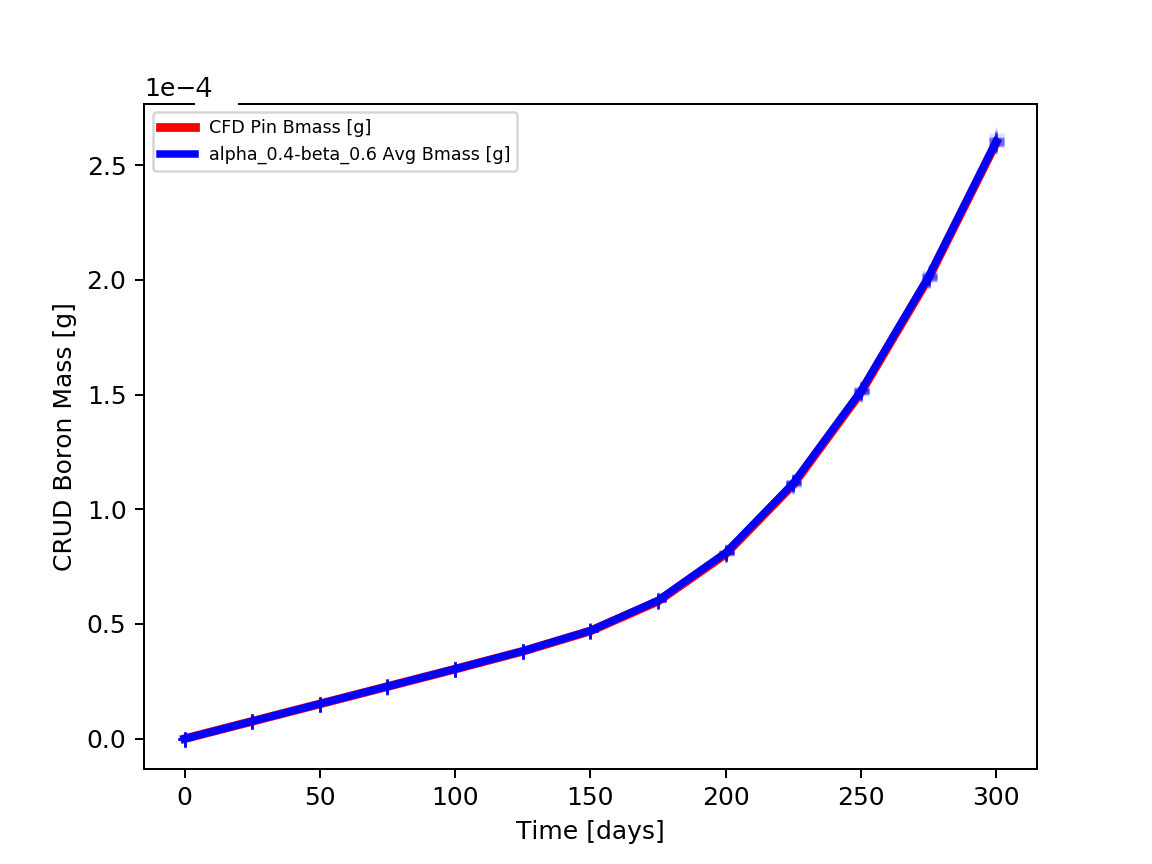
\includegraphics[width=0.7\linewidth]{figs/synth/cmpr_pin_totals_0_4_0_6}
    \caption[Total integrated crud boron mass vs. time using approximately optimal remapping weights.]{Total integrated crud boron mass vs. time using approximately optimal remapping weights ($w_T=0.4, w_{k}=0.6, w_{q''}=0.0$).}
    \label{fig:cmprpintotals0406}
\end{figure}
\begin{figure}[H]
    \centering
    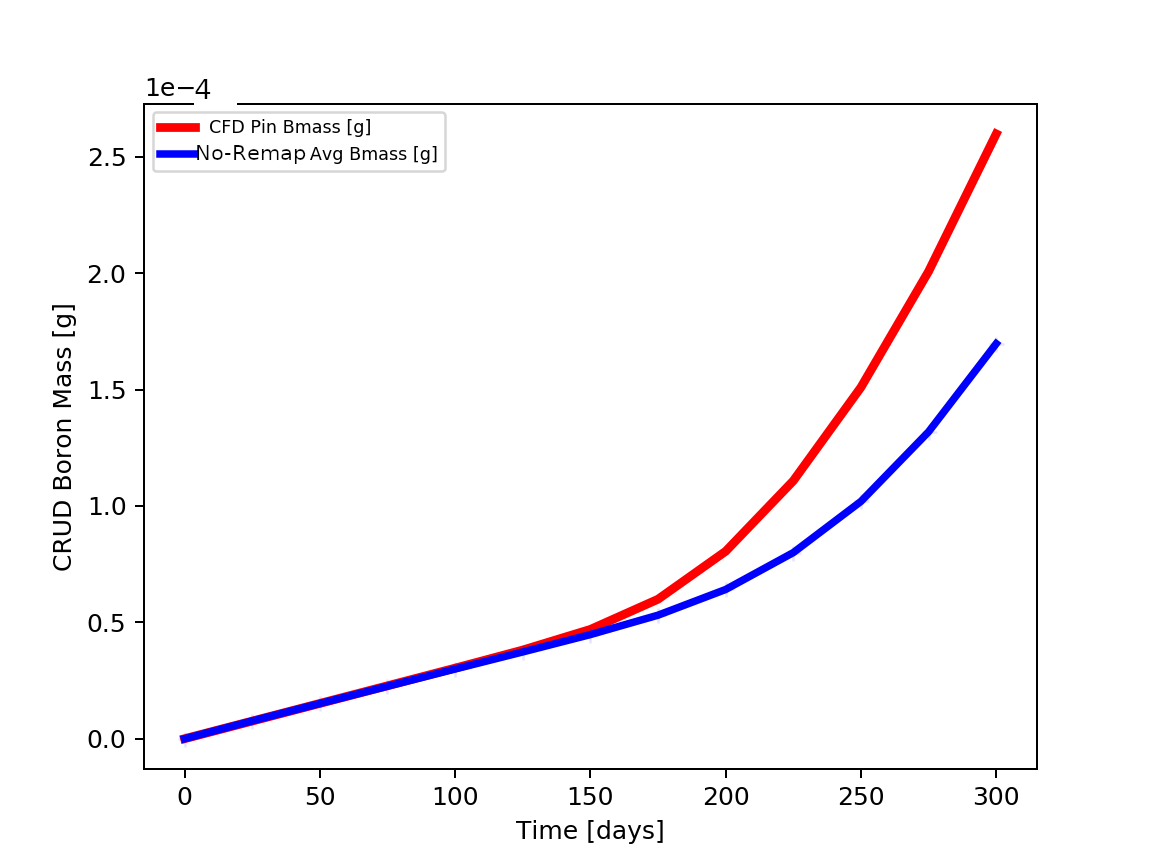
\includegraphics[width=0.7\linewidth]{figs/synth/cmpr_pin_totals_no_remap}
    \caption{Total integrated crud boron mass vs. time without remapping samples.}
    \label{fig:cmprpintotalsnoremap}
\end{figure}

A spatial representation of the samples pre and post-remapping are shown in figure \ref{fig:remmap_comp}.  A visual representation of the remapping strategy presented is presented in figure %\ref{fig:samplemapping}.  
While the spatial distribution of the temperature and TKE fields are distinctly different after the remapping procedure is applied, the joint density distributions formed by the sample population over the patch are identical.

\begin{figure}[H]%
    \centering
    \subfloat[Remapped surface samples.]{{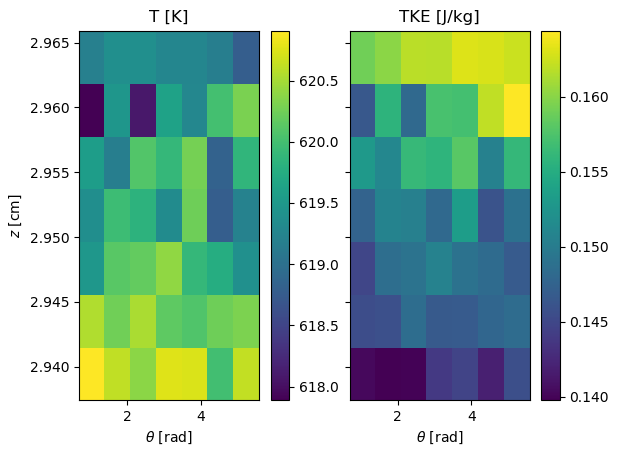
\includegraphics[width=0.53\linewidth]{figs/synth/patch_fields_0_4_0_6} }}\hspace*{-1.0em}%
    \subfloat[Non-remapped surface samples]{{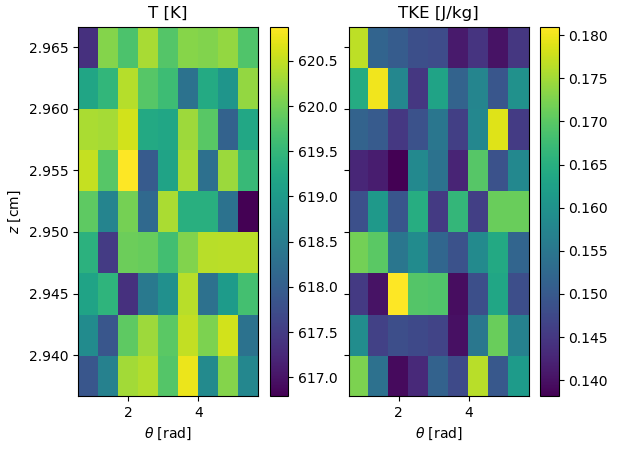
\includegraphics[width=0.53\linewidth]{figs/synth/patch_fields_no_remap} }}%
    \caption[Re-mapped and non-remapped temperature and TKE surface samples]{Re-mapped (a) and non remapped (b) temperature and TKE surface samples for a single CTF face.}%
    \label{fig:remmap_comp}%
\end{figure}

\subsection{Resample Frequency}
\label{sec:resample_freq_study}

The frequency at which the distribution functions are sampled from on each CTF face influences the variance in the predicted integrated crud results.  To investigate the behavior of the varience of the crud results as a function of resampling frequency, a parameter sweep was conducted in which crud was grown on the same pin with resampling time step sizes of 50, 100, and 300 $[days]$.  50 independent trials were conducted for each step size.  Shown in figure \ref{fig:cmprpintotalsviolin} a smaller resampling steps size, $\Delta t_s$, results in a reduction in the variance of the rod integrated crud estimates at 300 days of simulation time.   Additionally, the sampling induced rod integrated crud mass uncertainties were shown to be approximately distributed according to a normal distribution.  It is also important to note that the variance of the rod integrated crud results increases as a function of time.

\begin{figure}[H]
    \centering
    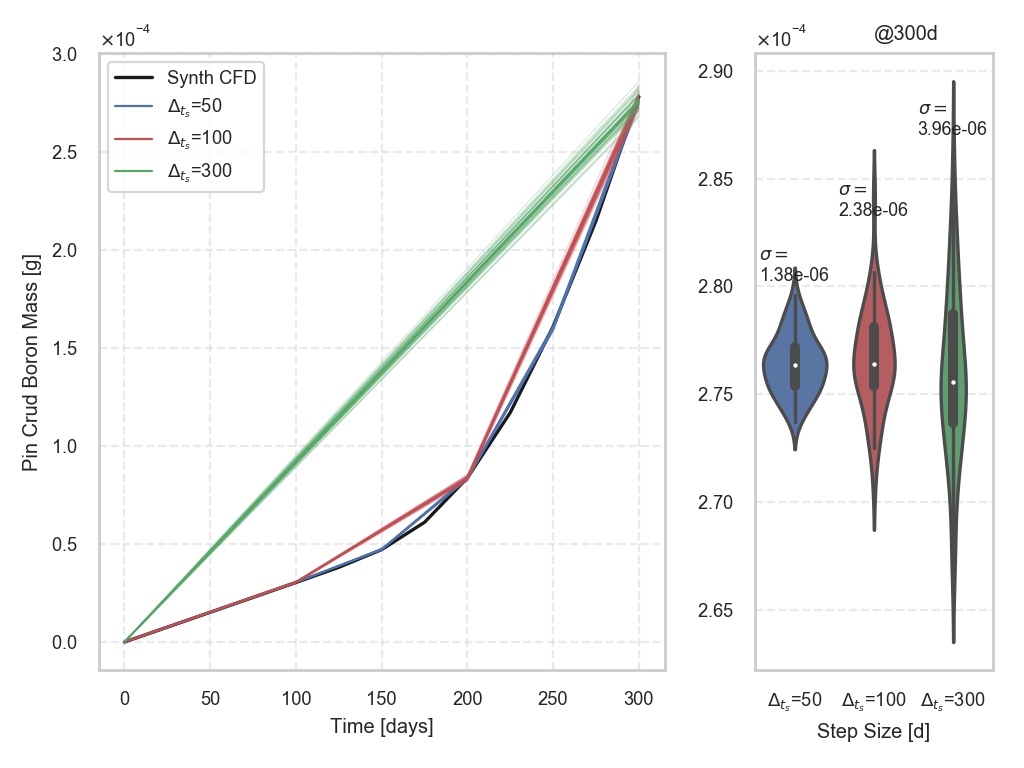
\includegraphics[width=0.7\linewidth]{figs/synth/tstep_study/cmpr_pin_totals_violin}
    \caption[Influence of the resample frequency on the predicted integrated crud variance.]{Influence of the resample frequency on the predicted rod integrated crud variance.  Crud variance estimates at 300 $[days]$ are given in the right hand side of the figure from 50 independent trials for each of the step size cases.}
    \label{fig:cmprpintotalsviolin}
\end{figure}

Performing a larger number of resampling events per VERA state results in reduced variance at little additional computational effort.
This is in part due to the minimal computational requirements of sampling the joint temperature and TKE distribution on each patch.  Drawing samples from a bivariate copula density model is straight forward and can be done in parallel since each patch is treated as an independent sampling zone in this hi2lo approach.  The crud computation, by comparison, is more expensive.  Increasing the resampling frequency does not increase the total number of samples used per pin per time step, rather, this process only increases the number of (resample) steps per VERA state point.  The reduction in variance stems from an improved sample density throughout time of the underlying random field.  In time, the underlaying random field is fixed throughout a VERA state point.  Repeatedly drawing samples from this field at small time steps rather than sampling the random field only once at the beginning of the VERA state point vastly increases the number of samples used to perform the time integration of the crud result on each CTF face.


\section{Section Takeaways}
\begin{itemize}
        \item  Good rod integrated crud agreement between the synthetic source data and the predicted results was observed.  The rod integrated results were summarized in table \ref{tab:crud_totals_2}.  Fitting copula and marginal distributions to the sample data, resampling from these models, and then growing curd using these samples reproduces the correct total amount of crud at each time step and correctly reproduces the axial distribution of crud as shown in figure \ref{fig:hi2lopincmass}.
        \item Increasing the number of samples drawn per CTF patch decreases variance in total crud mass and total precipitated boron estimates.  The number of samples used is an adjustable runtime parameter and can be increased depending on the available computational resources and accuracy desired.
        \item Increasing the number of resampling steps per VERA state point reduces variance in the final integrated crud results. 
        \item After drawing samples from the joint density distribution a reordering of the samples on the rod surface is necessary to preserve hot spot stationarity.  Demonstrated in figure \ref{fig:cmprpintotals0406} and \ref{fig:cmprpintotalsnoremap}, sample remapping with weights of $w_T=0.4,\ w_k=0.6$ was performed to achieve an optimal time marching sampling strategy.
        \item Importance sampling was shown to reduce the variance in the integrated crud results.
        \item A synthetic data generation tool allows absolute control over the properties of joint distribution of TH boundary conditions which are fed into the crud simulation code.  Since the synthetic data has known statistical properties, this data serves as an important data source for benchmarking and validation operations.
\end{itemize}
